\documentclass[a4paper,11pt]{article}
\author{ 杨旭鹏  \  PB17000234}
\date{2019年秋季}
\title{计算物理A 第七题}

\usepackage{ctex}
\usepackage{amsmath}
\usepackage{amsfonts}
\usepackage{graphicx}
\usepackage{lastpage}
\usepackage{hyperref}
\usepackage{listings}
\RequirePackage{xcolor}
\usepackage{appendix}
\makeatletter\def\@captype{table}\makeatother
\definecolor{dkgreen}{rgb}{0,0.6,0}
\definecolor{gray}{rgb}{0.5,0.5,0.5}
\definecolor{mauve}{rgb}{0.58,0,0.82}


\lstset{
  frame=tb,
  aboveskip=3mm,
  belowskip=3mm,
  showstringspaces=false,
  columns=flexible,
  framerule=1pt,
  rulecolor=\color{gray!35},
  backgroundcolor=\color{gray!5},
  basicstyle={\small\ttfamily},
  numbers=left,
  numberstyle=\tiny\color{gray},
  keywordstyle=\color{blue},
  commentstyle=\color{dkgreen},
  stringstyle=\color{mauve},
  breaklines=true,
  breakatwhitespace=true,
  tabsize=3,            
  }



\begin{document}
\maketitle

\section{题目描述}
对一个实验谱数值曲线 $p(x)$ ,自设 $F(x)$,分别用直接抽样和舍选法 对 $p(x)$ 抽样。比较原曲线和抽样得到的曲线以验证。讨论抽样效率。

\section{算法及程序思路}
\subsection{算法}
由于指定的数据文件“data.txt”为离散分布的,故我们这里采用离散抽样。
\subsection{直接抽样}
由“data.txt”文件我们看到,横坐标能量(eV)$\in [2900,3013]$共114个取值。对于其中某一数据点$x_{i}$,其对应纵坐标值(即数目)为$n_{i}$,则对于某一次随机抽样,其为$x_{i}$的概率为$p_{i} = \frac{n_{i}}{\sum^{n-1}_{i=1}n_{i}}$。

其直接抽样方法为:在$[0,1]$间由均匀抽样抽取一值$\xi$,若$\sum^{k}_{i=1}p_{i}<\xi\leq \sum^{k+1}_{i=1}p_{i}$,则其横坐标能量$x$的取值为$x_{k}$。

\subsection{舍选法抽样}
观察“data.txt”中给出的数据,我们发先在$x \leq 2994$时计数量相对平稳,其内的概率最大值为在$x=2965$处取得的约0.0144(对应原数据计数5672)。而在$x \in [2995,3005]$时有一个峰,其概率峰值在3001处取得约0.0951(对应原数据计数37630)。而在之后$x$对应的概率比较小(概率$<0.00253$,对应原数据计数$<1000$)。故我们可采取较为简单的分段函数来作为比较函数进行舍选法抽样。

在此题中所使用的比较函数$F(x)$为:
\begin{equation}
F(x) = 
\left\{
\begin{array}{l}
	0.0144 ~~~~~~,x \in [2900,2994) \\
	0.0951 ~~~~~~,x \in [2994,3005) \\
	0.00253 ~~~~ ,x \in [3005,3013]
\end{array}
\right.
\end{equation}

\begin{figure}[!htbp]        
\center{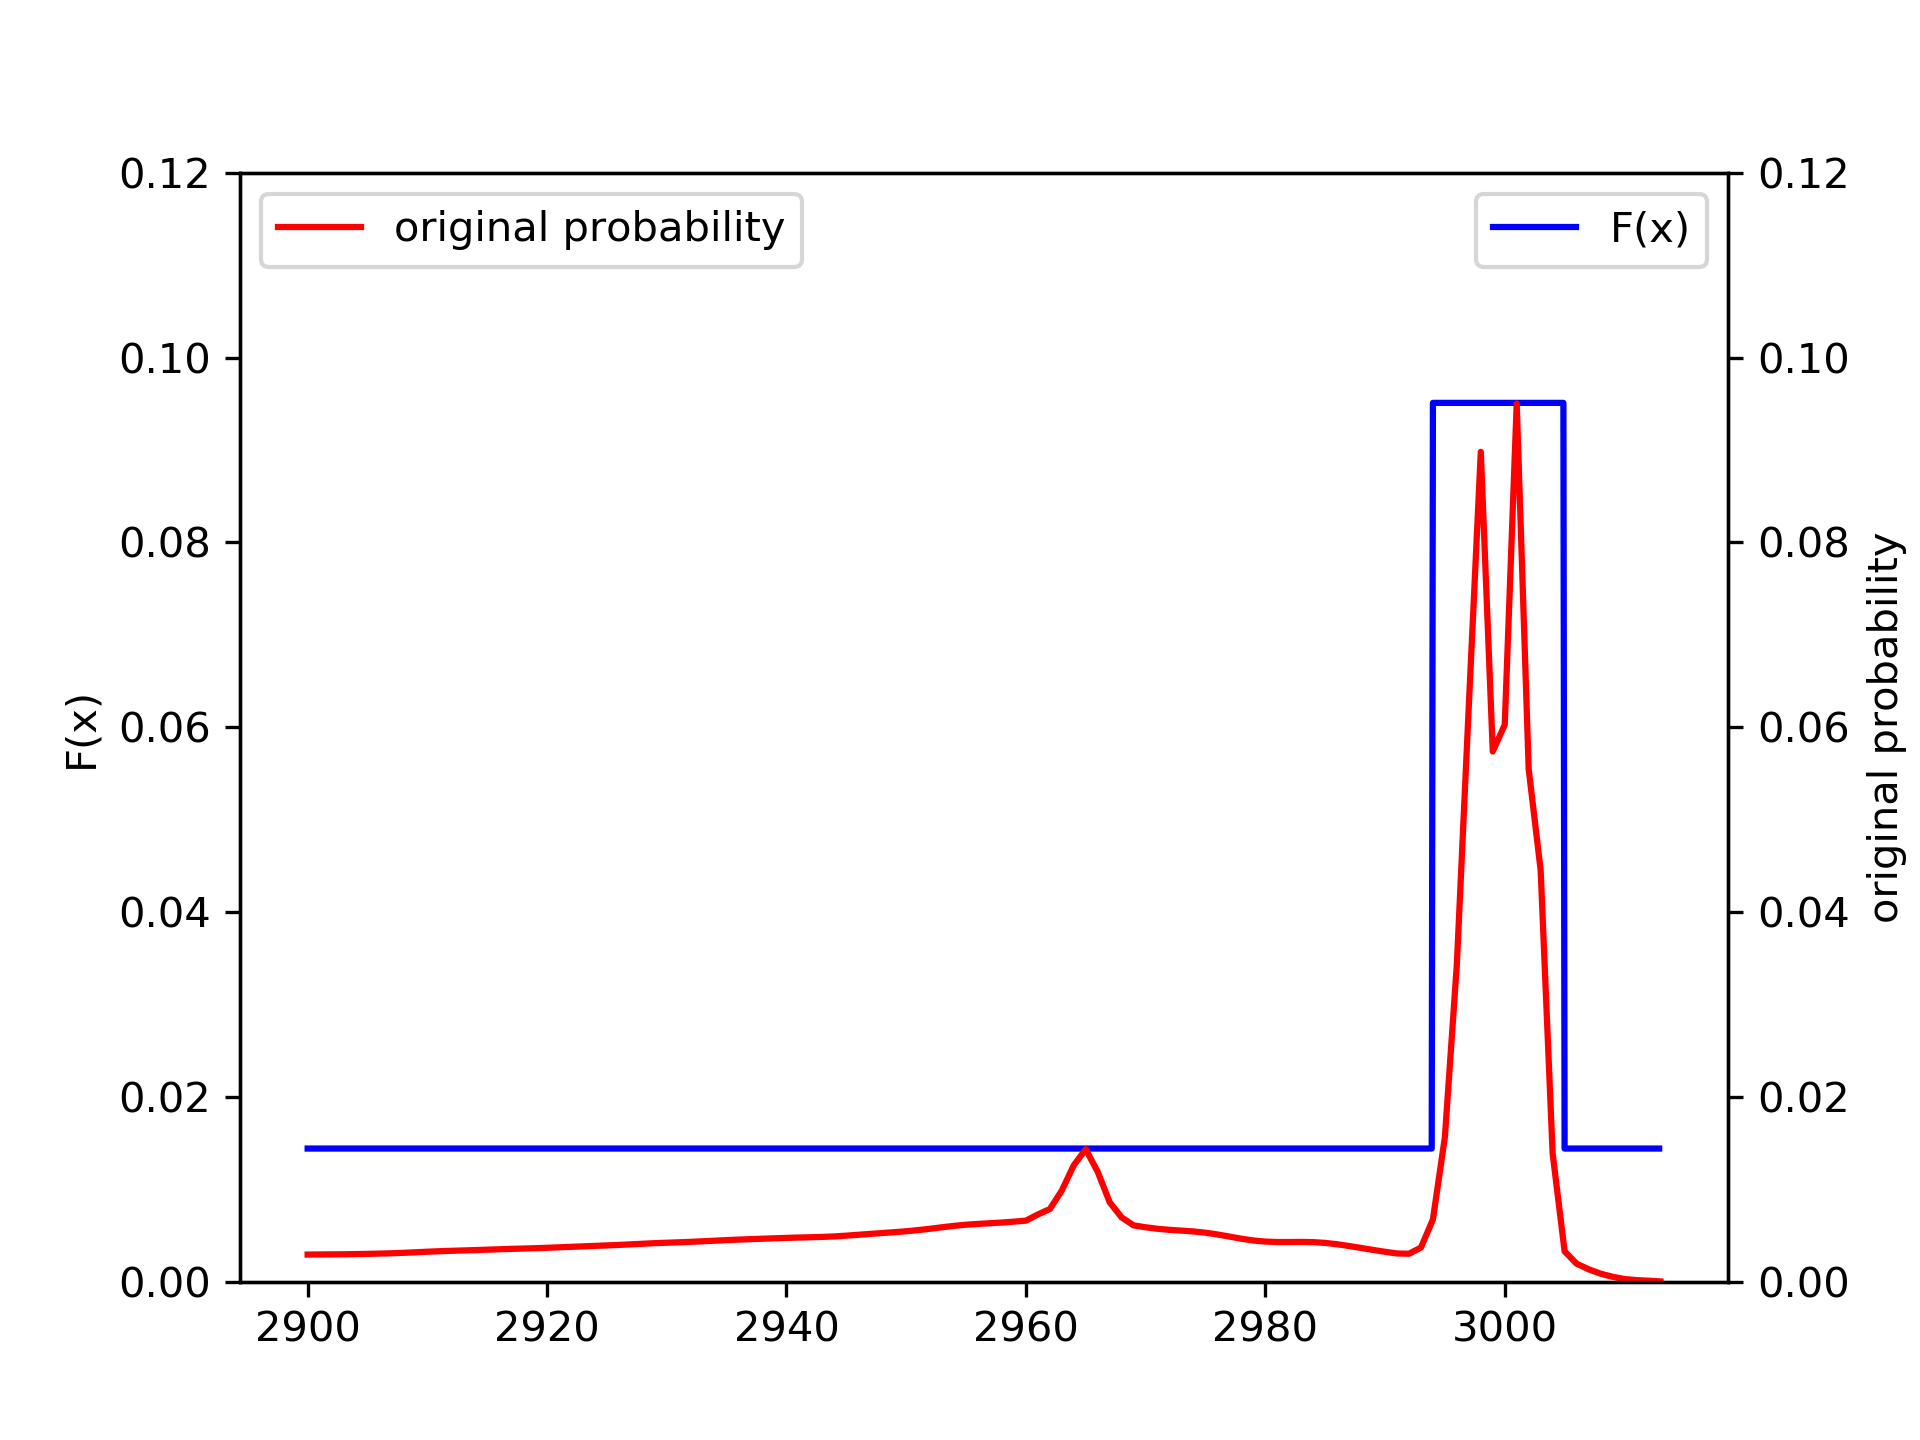
\includegraphics[width=10cm]  {F(x).png}}        
\caption{\label{1} 比较函数与给定概率分布的比较}      
\end{figure}

其累积函数$\xi(x)$为:
\begin{equation}
	\xi(x)=
\left\{
\begin{array}{l}
	0.0144(x-2900) ~~~~~~,x \in [2900,2994) \\
	0.0951(x-2994) + 1.3536 ~~~~~~,x \in [2994,3005) \\
	0.00253(x-3005) + 1.0461 + 1.3536  ~~~~ ,x \in [3005,3013]
\end{array}
\right.
\end{equation}
可知$\xi(x) \in [0,2.41994]$,则可取反函数$x(\xi)$:\footnote{其中$floor()$表示向下取整的函数}

\begin{equation}
x(\xi) = 
\left\{
\begin{array}{l}
 floor(\frac{\xi}{0.0144} +2900) ~~~~~~,\xi \in [0,1.3536]  \\
 floor(\frac{\xi-1.3536}{0.0951}+2994) ~~~~~~,\xi \in [1.3536,1.0461 + 1.3536]  \\
 floor(\frac{\xi-1.3536-1.0461}{0.00253}+3005)~~~~~~,\xi \in [1.0461 + 1.3536,0.02024+1.0461 + 1.3536]

\end{array}
\right.
\end{equation}

化简即:

\begin{equation}
x(\xi) = 
\left\{
\begin{array}{l}
 floor(\frac{\xi}{0.0144} +2900) ~~~~~~,\xi \in [0,1.3536]  \\
 floor(\frac{\xi-1.3536}{0.0951}+2994) ~~~~~~,\xi \in [1.3536,2.3997]  \\
 floor(\frac{\xi-2.3997}{0.00253}+3005)~~~~~~,\xi \in [2.3997,2.41994]
\end{array}
\right.
\end{equation}
其中,$\xi$为$[0,2.41994]$间均匀抽取的随机数。

对于属于不同区间的$\xi$值,我们均匀抽取在不同区间的随机数$\eta$:
\begin{equation}
\left\{
\begin{array}{l}
 \eta \in [0,0.0144]~~~~~~,\xi \in [0,1.3536]  \\
 \eta \in [0,0.0951] ~~~~~~,\xi \in [1.3536,2.3997]  \\
 \eta \in [0,0.00253] ~~~~~~,\xi \in [2.3997,2.41994]
\end{array}
\right.
\end{equation}
则判断$\eta$是否小于对应$x(\xi)$数据的给定概率$p_{i}$。若是,则取此$x(\xi)$为抽取结果;不是则舍。


\subsection{16807产生器}
16807产生器属于线性同余法产生器的特例。而线性同余法方法为:

\begin{equation}
\begin{aligned}
	I_{n+1} &= (aI_{n} + b) \ mod \ m \\
	x_{n} &= I_{n}/m
\end{aligned}
\label{linear}	
\end{equation}

其中整数$I_{i} \in [0,m-1]$,$a,b,m$为算法中的可调参数,其选取直接影响产生器的质量。选取参数:
\begin{equation}
\left\{
\begin{array}{l}
	a = 7^{5} = 16807 \\
	b = 0 \\
	m = 2^{31}-1 = 2147483647
\end{array}
\right.
\end{equation}

即为所谓的16807产生器。由于直接利用\ref{linear}编写程序时计算$(aI_{n} \ mod \ m )$时很容易造成数据溢出,故采取Schrage方法进行具体编程的实现:

\begin{equation}
	aI_{n} \ mod \ m = \left\{
	\begin{array}{l}
		a(I_{n}\ mod \ q) - r[I_{n}/q],\ \ \ \ \ \ \ \ if \geq 0 \\
		a(I_{n}\ mod \ q) - r[I_{n}/q] + m,\ \ otherwise	
			\end{array}
	\right.
\end{equation}

其中$m=aq+r$,即$q=m/a=127773$,$r=m \ mod \ a=2836$。即可利用此方法产生伪随机数序列。



\section{程序使用方法}
在运行程序后,会自动输出“data.txt”中每一能量值对应的出现概率到“p.txt”。会看到请求输入所需总随机点数的提示,按照提示在后面输入所需要的总随机点数,摁回车继续。然后经过计算会分别给出直接抽样法和舍选法得到的数据到相应的文件。并在屏幕上输出舍选法的抽样效率。程序输出完这些后会自动退出。

\begin{figure}[!htbp]        
\center{
\includegraphics[width=7cm]  {example.png}}        
\caption{\label{1} 一个典型程序的运行过程示例}      
\end{figure}


\section{程序结果与讨论}
对于直接抽样法,我们有:

\begin{figure}[!htbp]        
\center{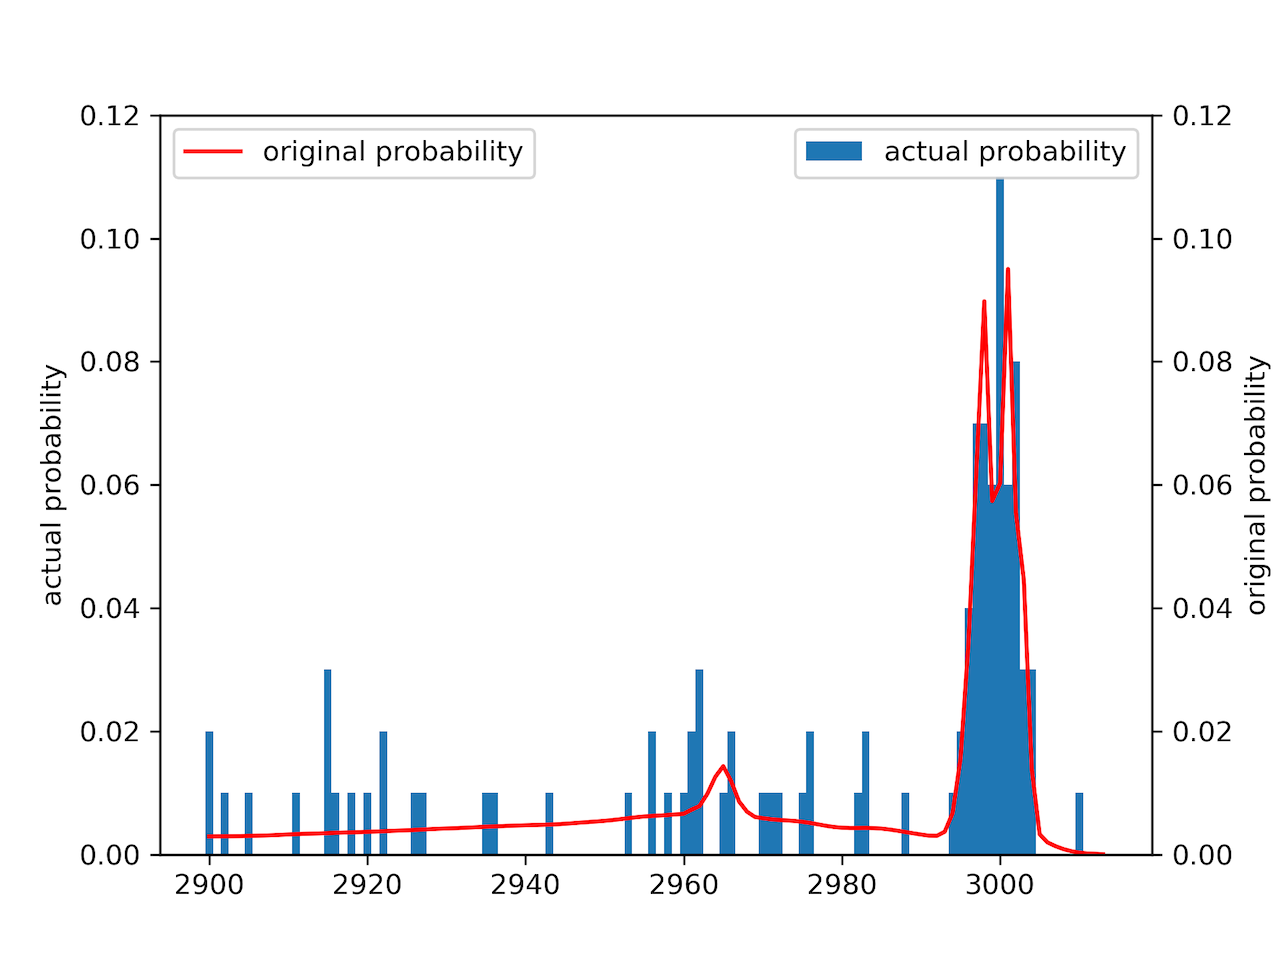
\includegraphics[width=10cm]  {102.png}}        
\caption{\label{1} 直接抽样$10^{2}$个点得到的概率分布与给定分布的比较}      
\end{figure}

\begin{figure}[!htbp]        
\center{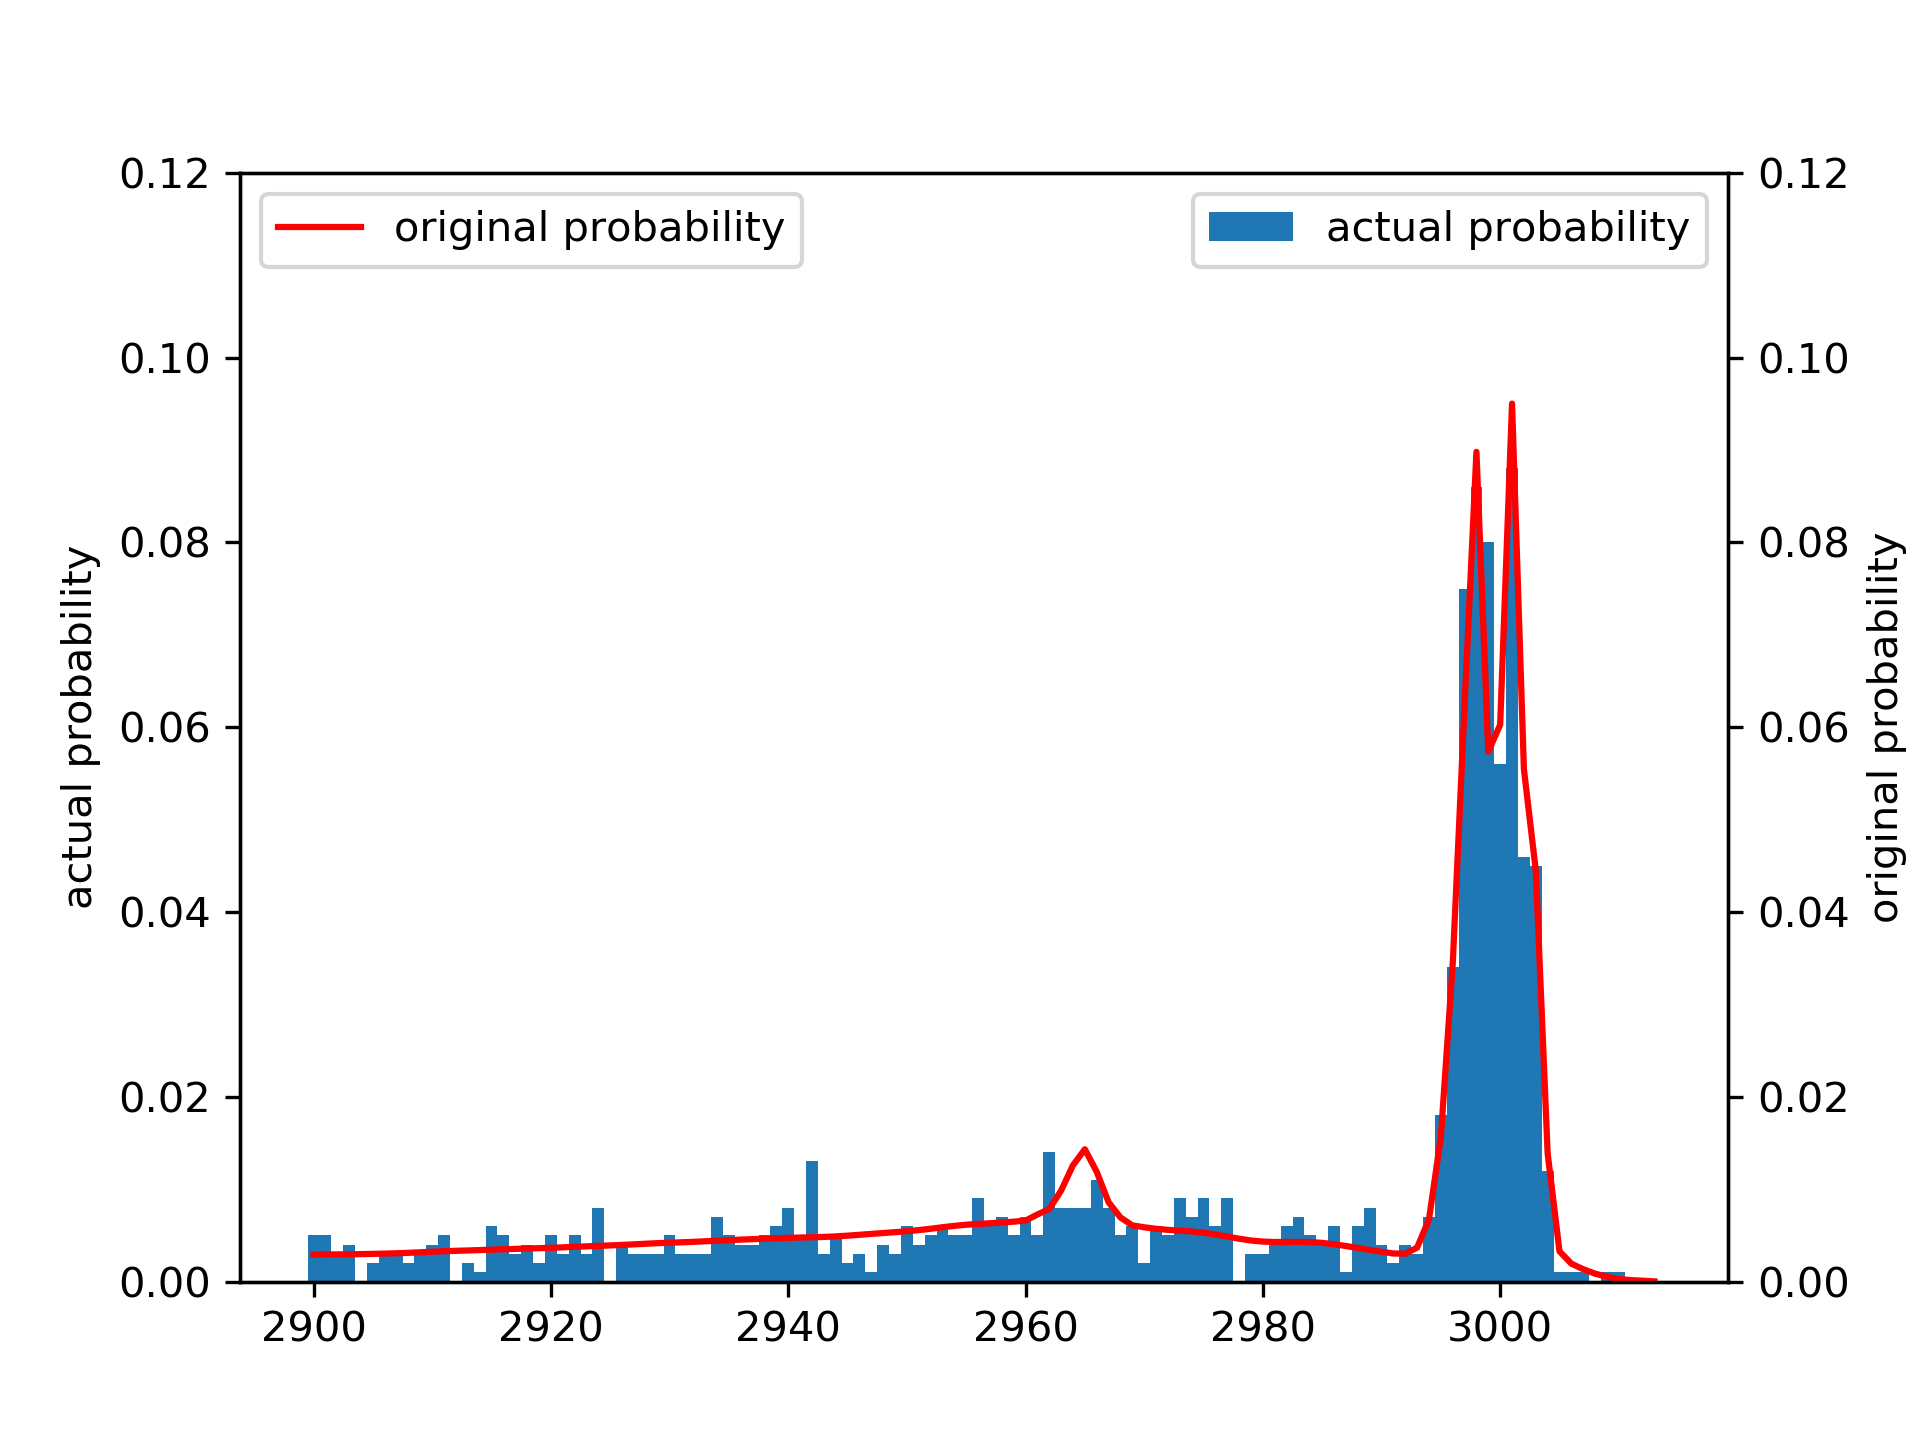
\includegraphics[width=10cm]  {103.png}}        
\caption{\label{1} 直接抽样$10^{3}$个点得到的概率分布与给定分布的比较}      
\end{figure}

\begin{figure}[!htbp]        
\center{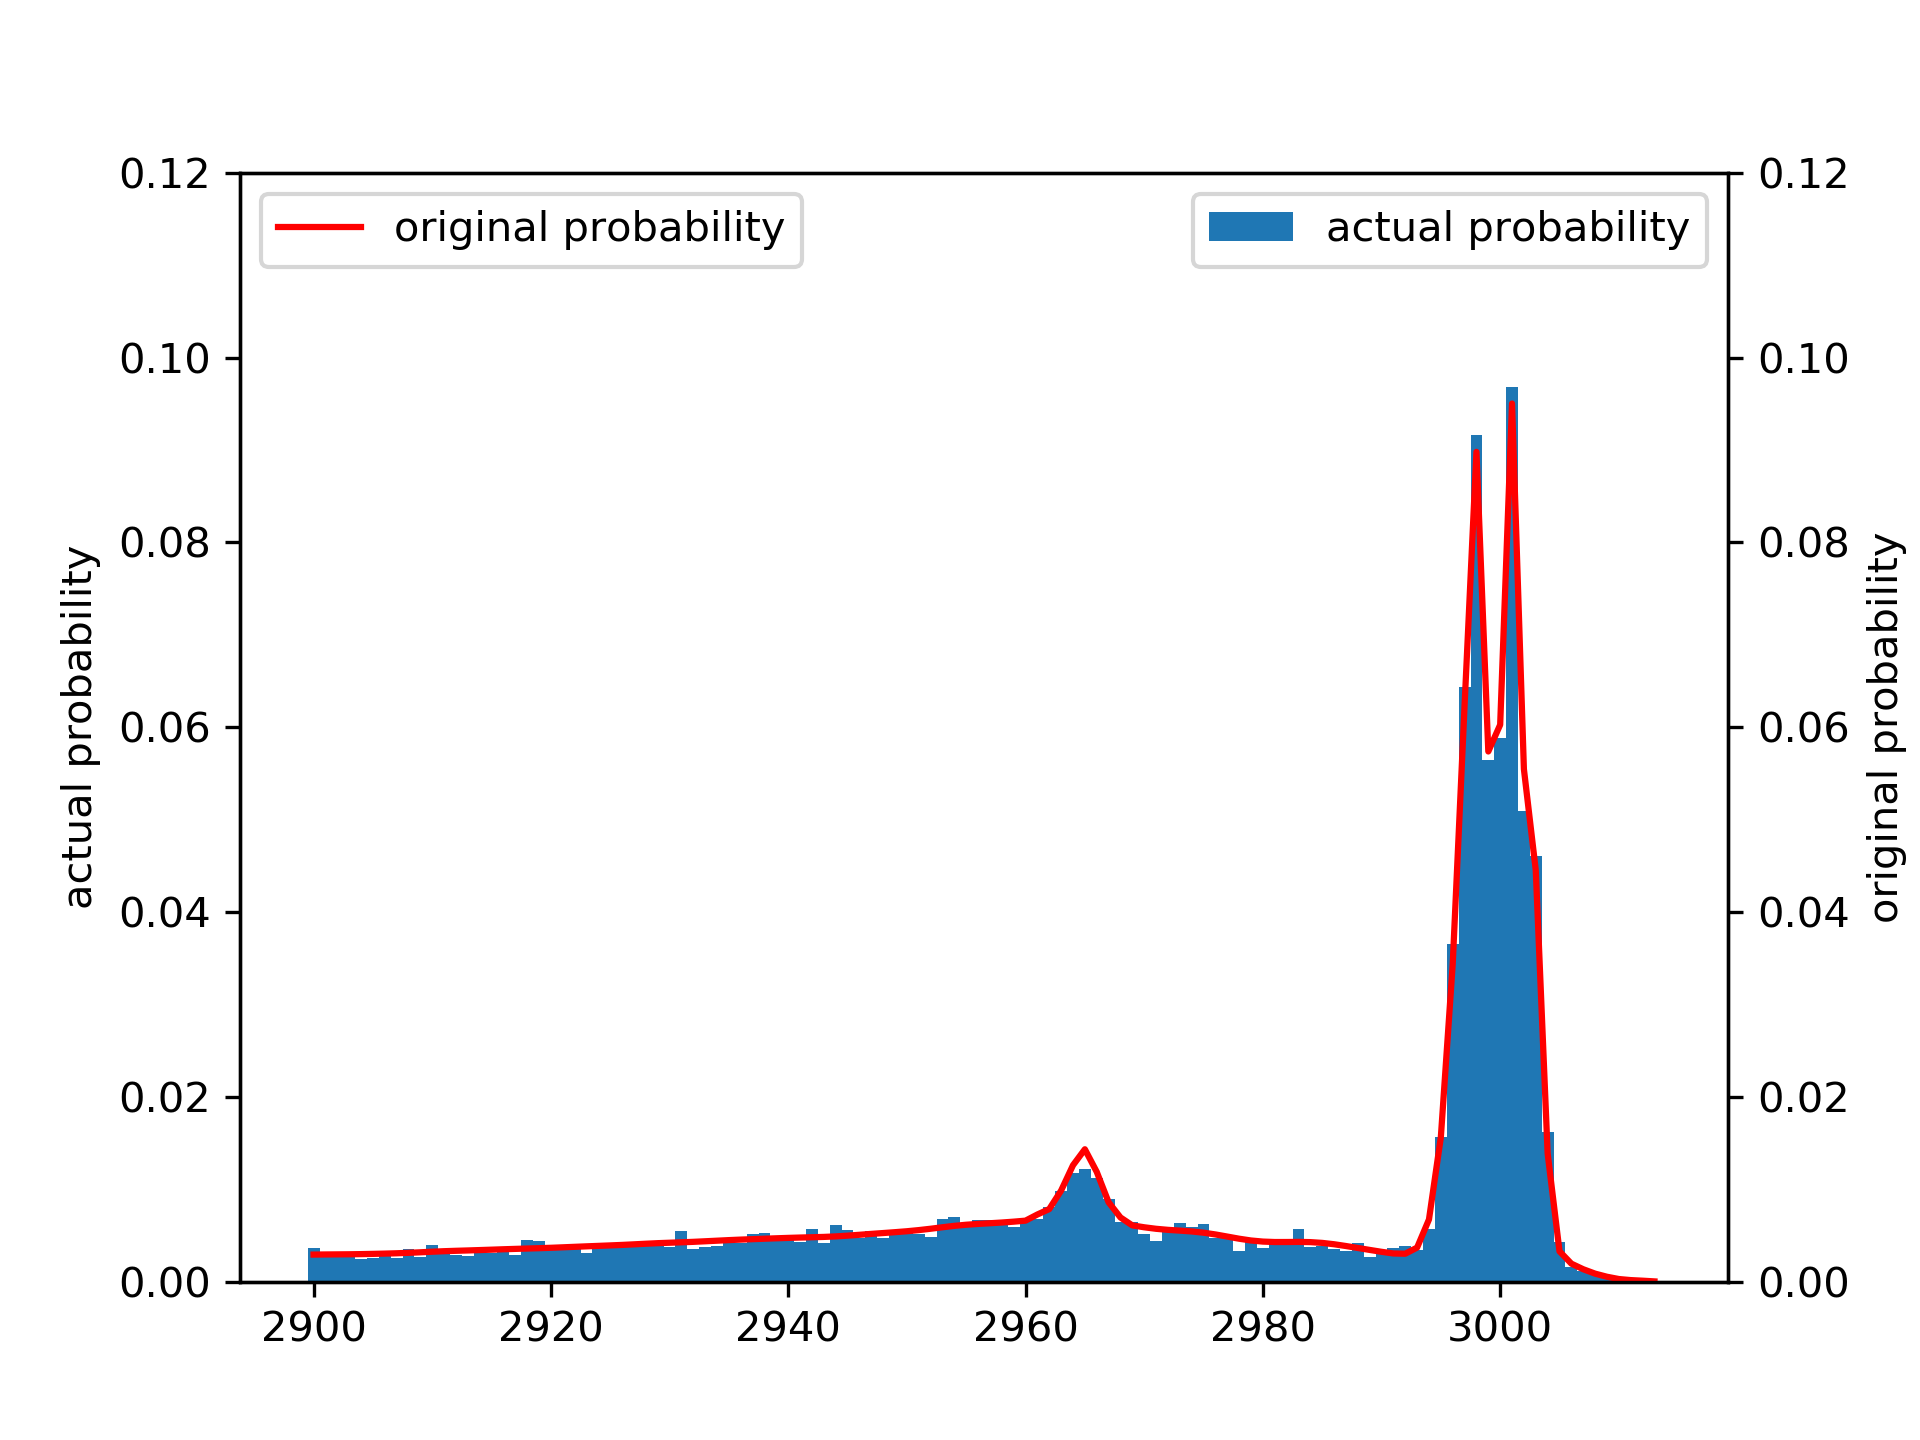
\includegraphics[width=10cm]  {104.png}}        
\caption{\label{1} 直接抽样$10^{4}$个点得到的概率分布与给定分布的比较}      
\end{figure}

\begin{figure}[!htbp]        
\center{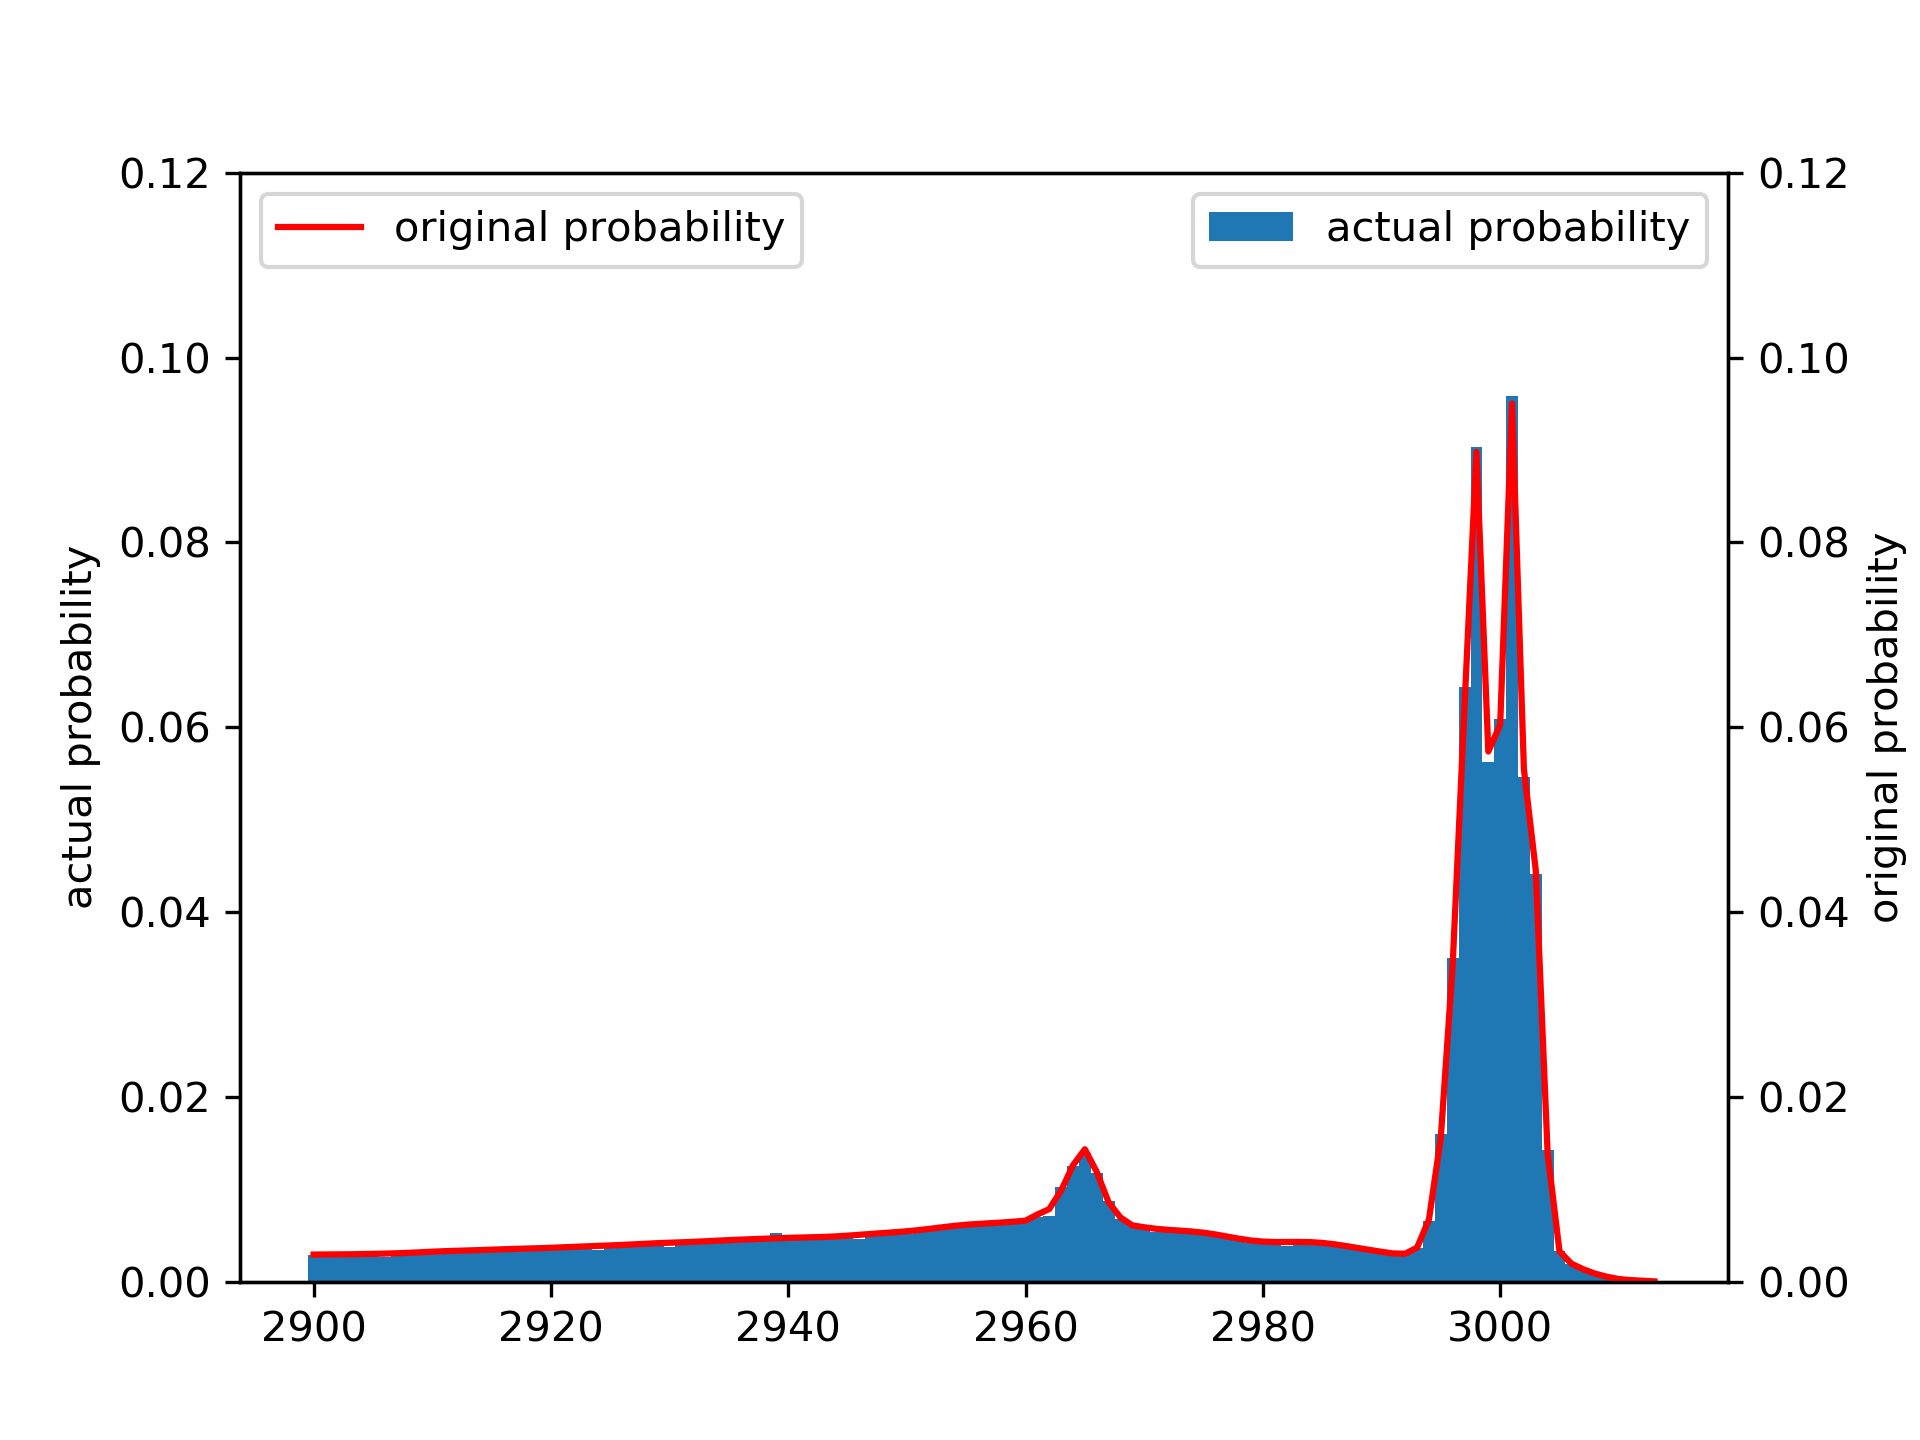
\includegraphics[width=10cm]  {105.png}}        
\caption{\label{1} 直接抽样$10^{5}$个点得到的概率分布与给定分布的比较}      
\end{figure}

\begin{figure}[!htbp]        
\center{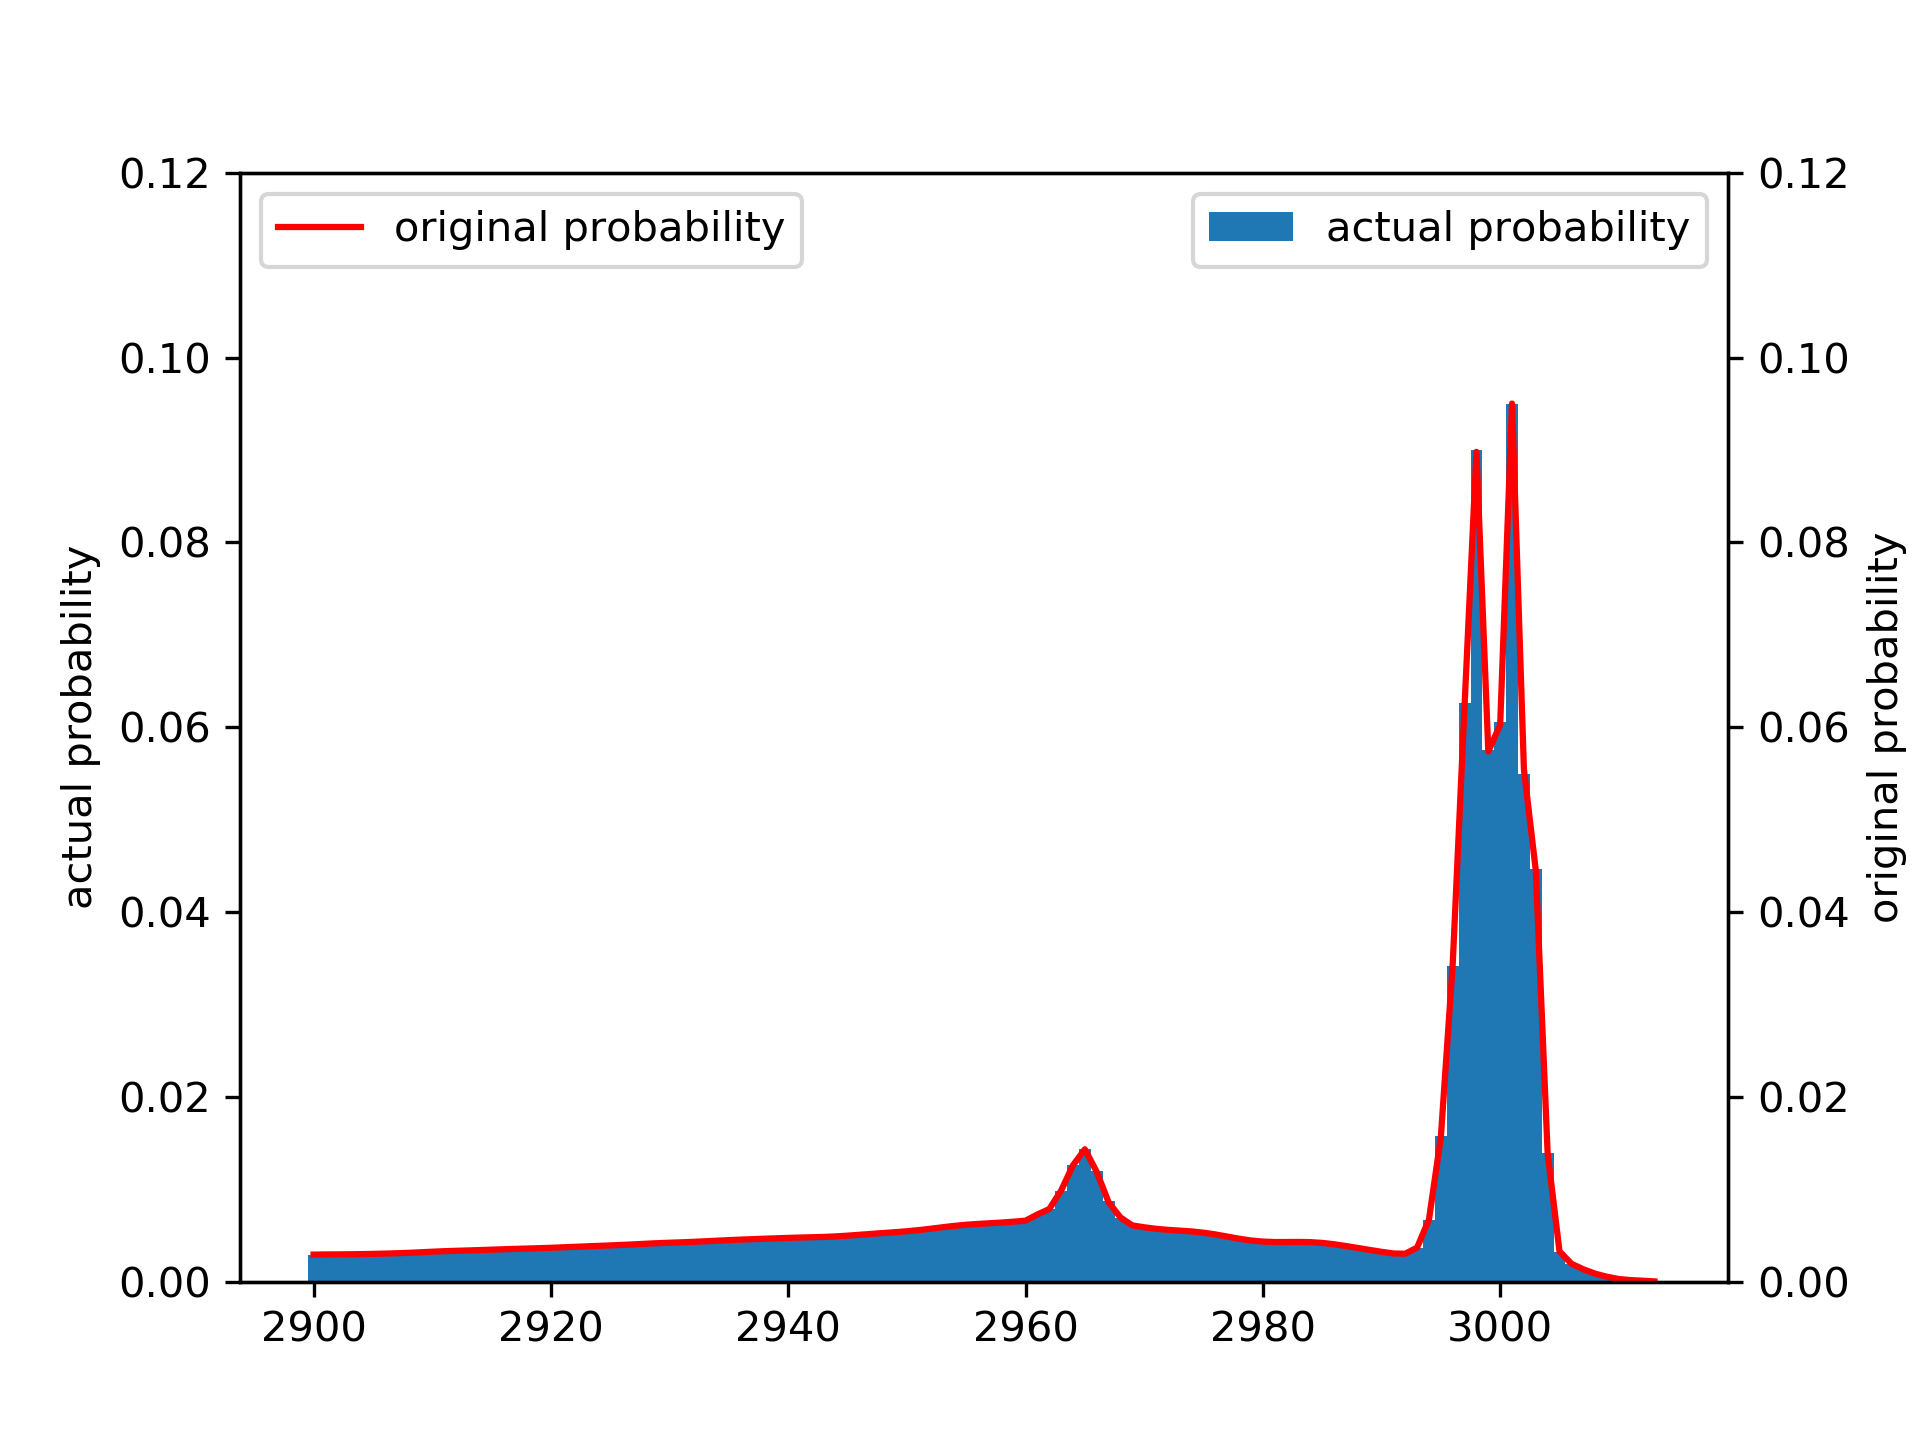
\includegraphics[width=10cm]  {106.png}}        
\caption{\label{1} 直接抽样$10^{6}$个点得到的概率分布与给定分布的比较}      
\end{figure}

\begin{figure}[!htbp]        
\center{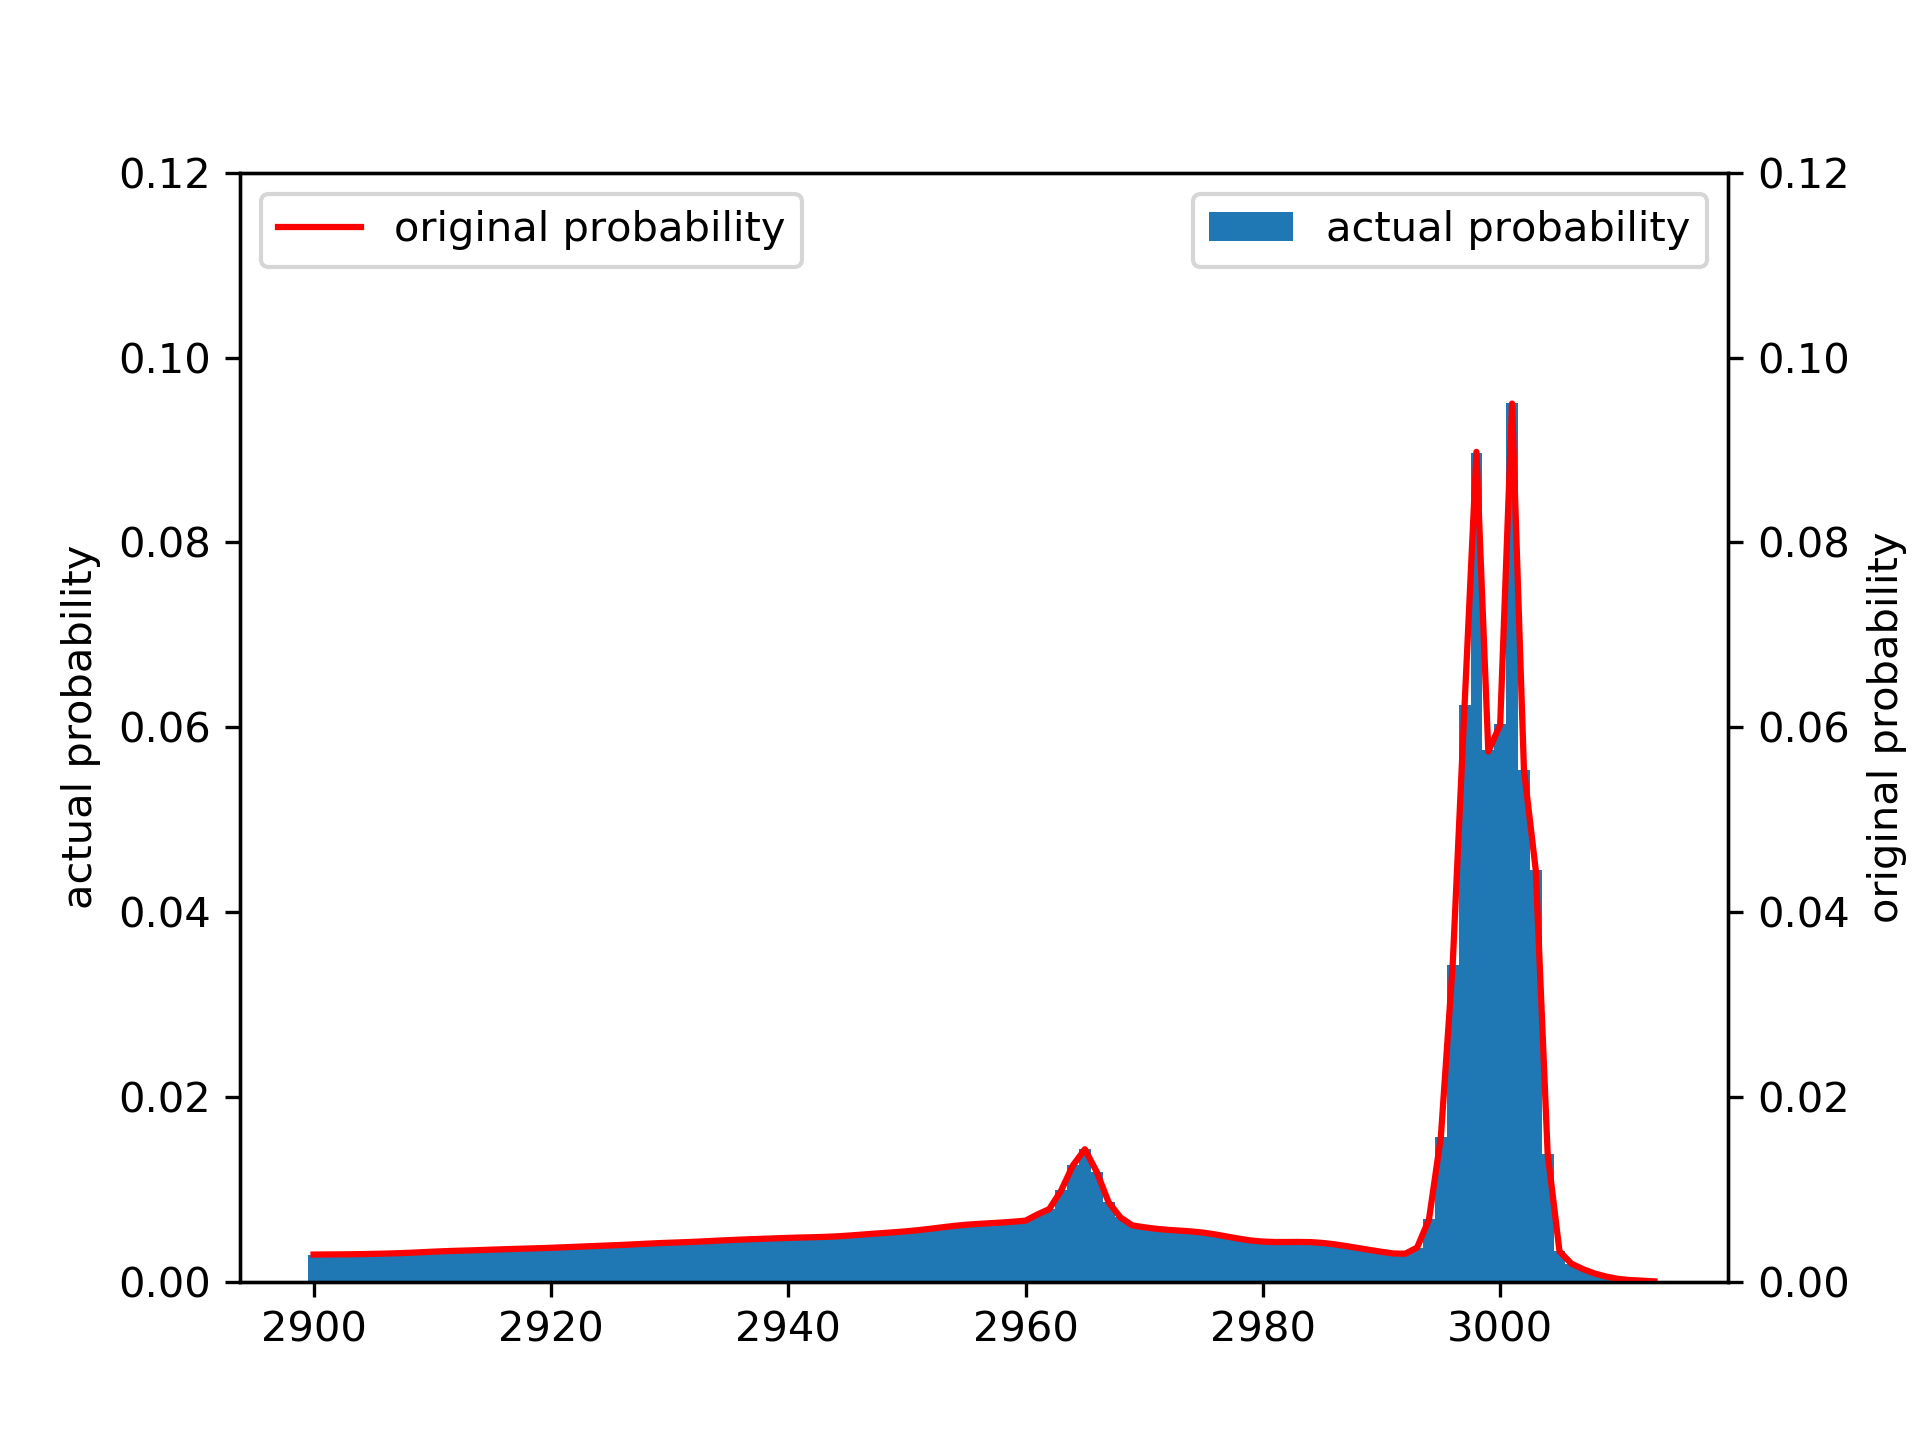
\includegraphics[width=10cm]  {107.png}}        
\caption{\label{1} 直接抽样$10^{7}$个点得到的概率分布与给定分布的比较}      
\end{figure}

\newpage 对于舍选法,得到:

\begin{figure}[!htbp]        
\center{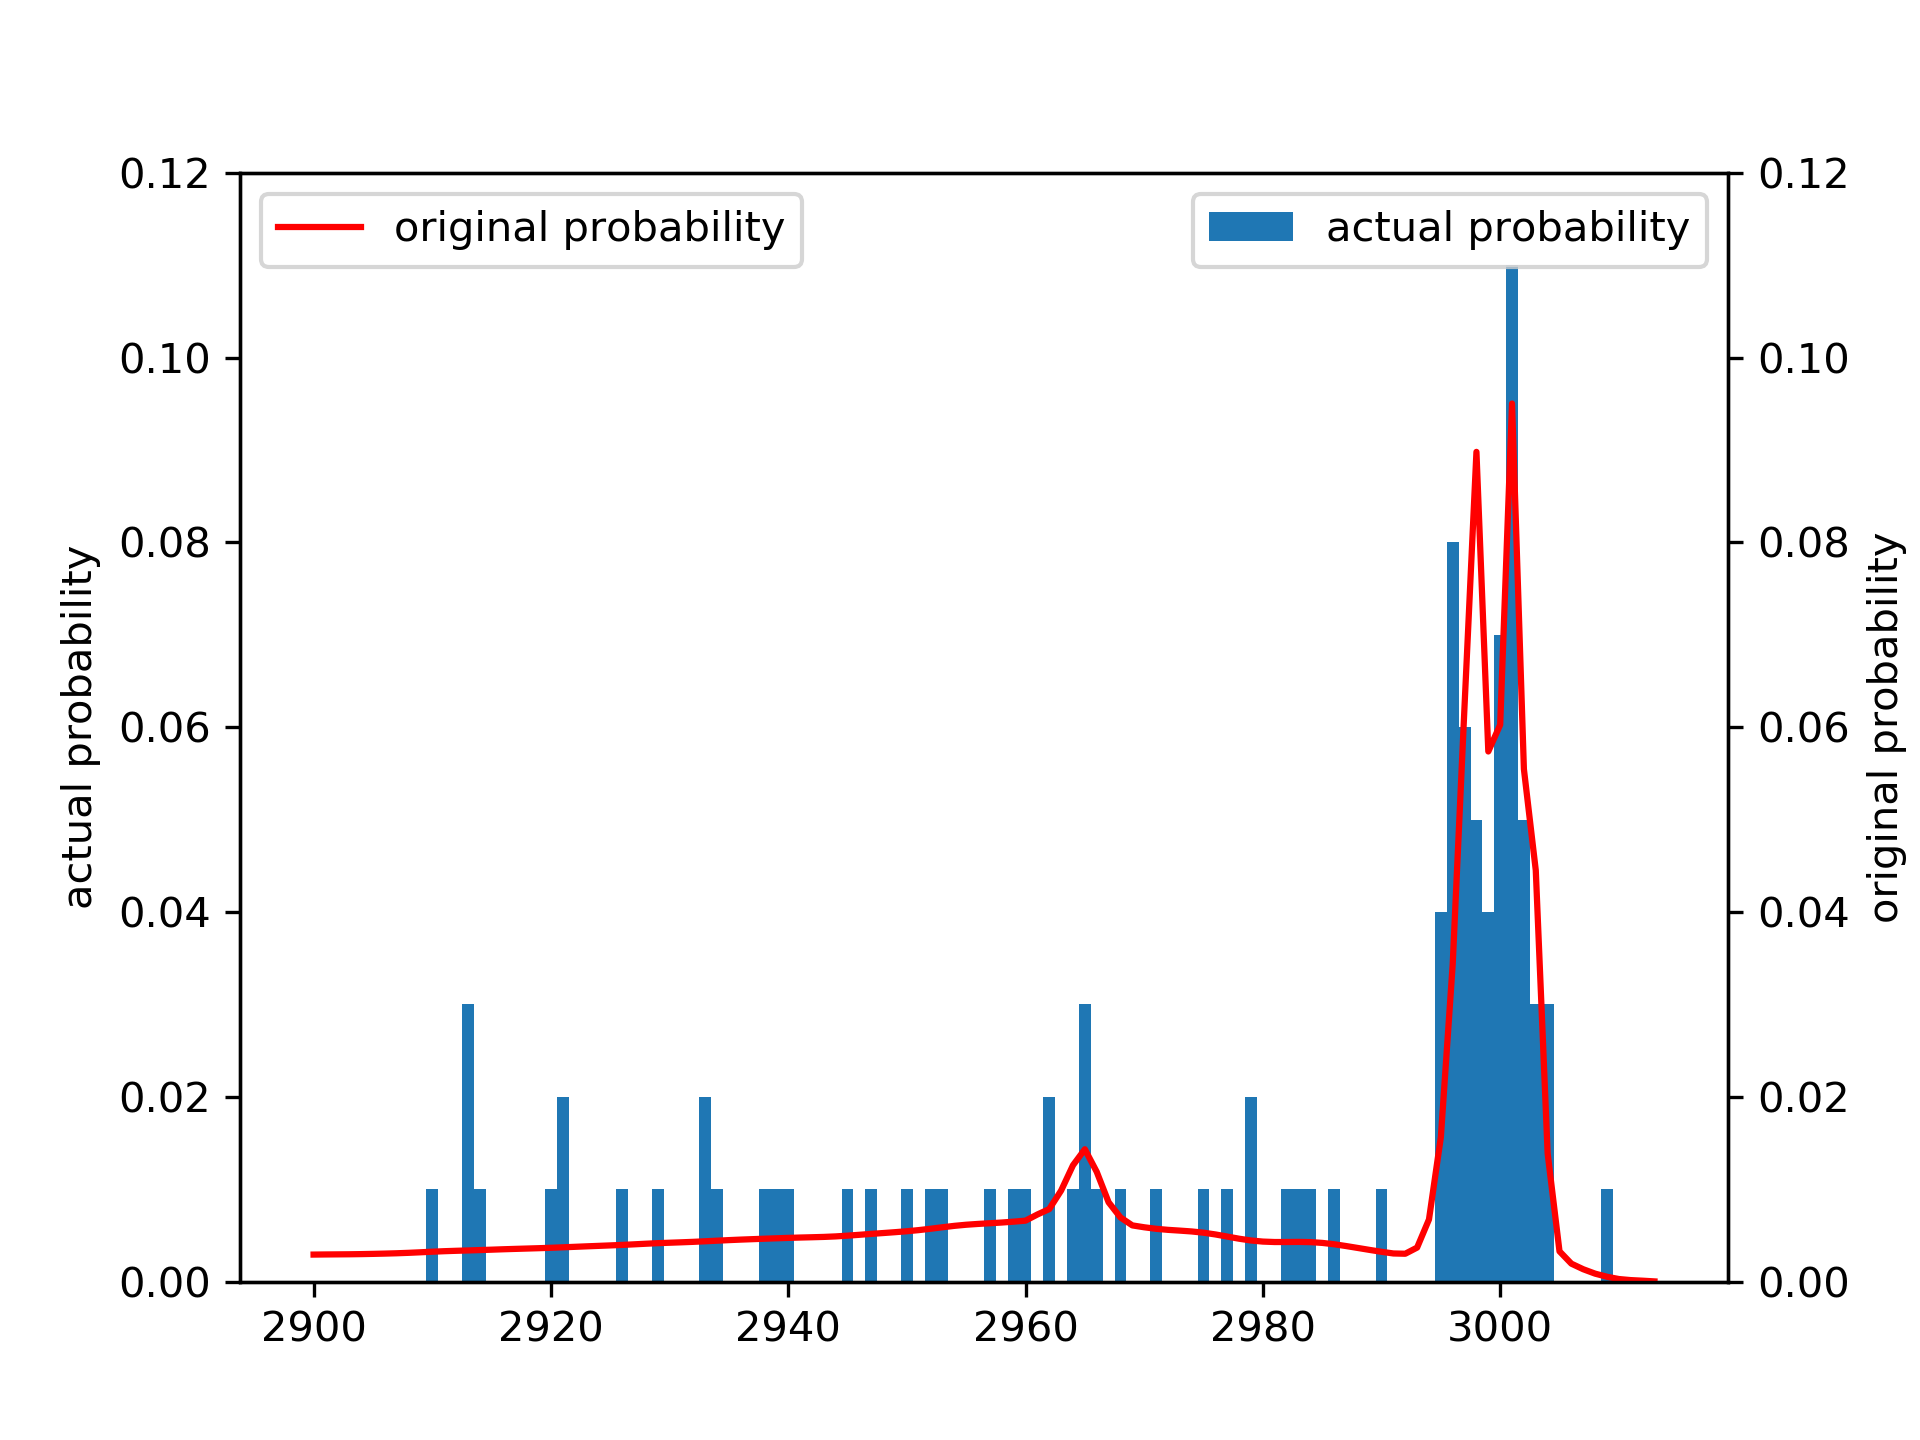
\includegraphics[width=10cm]  {c102.png}}        
\caption{\label{1} 舍选法$10^{2}$个点得到的概率分布与给定分布的比较}      
\end{figure}

\begin{figure}[!htbp]        
\center{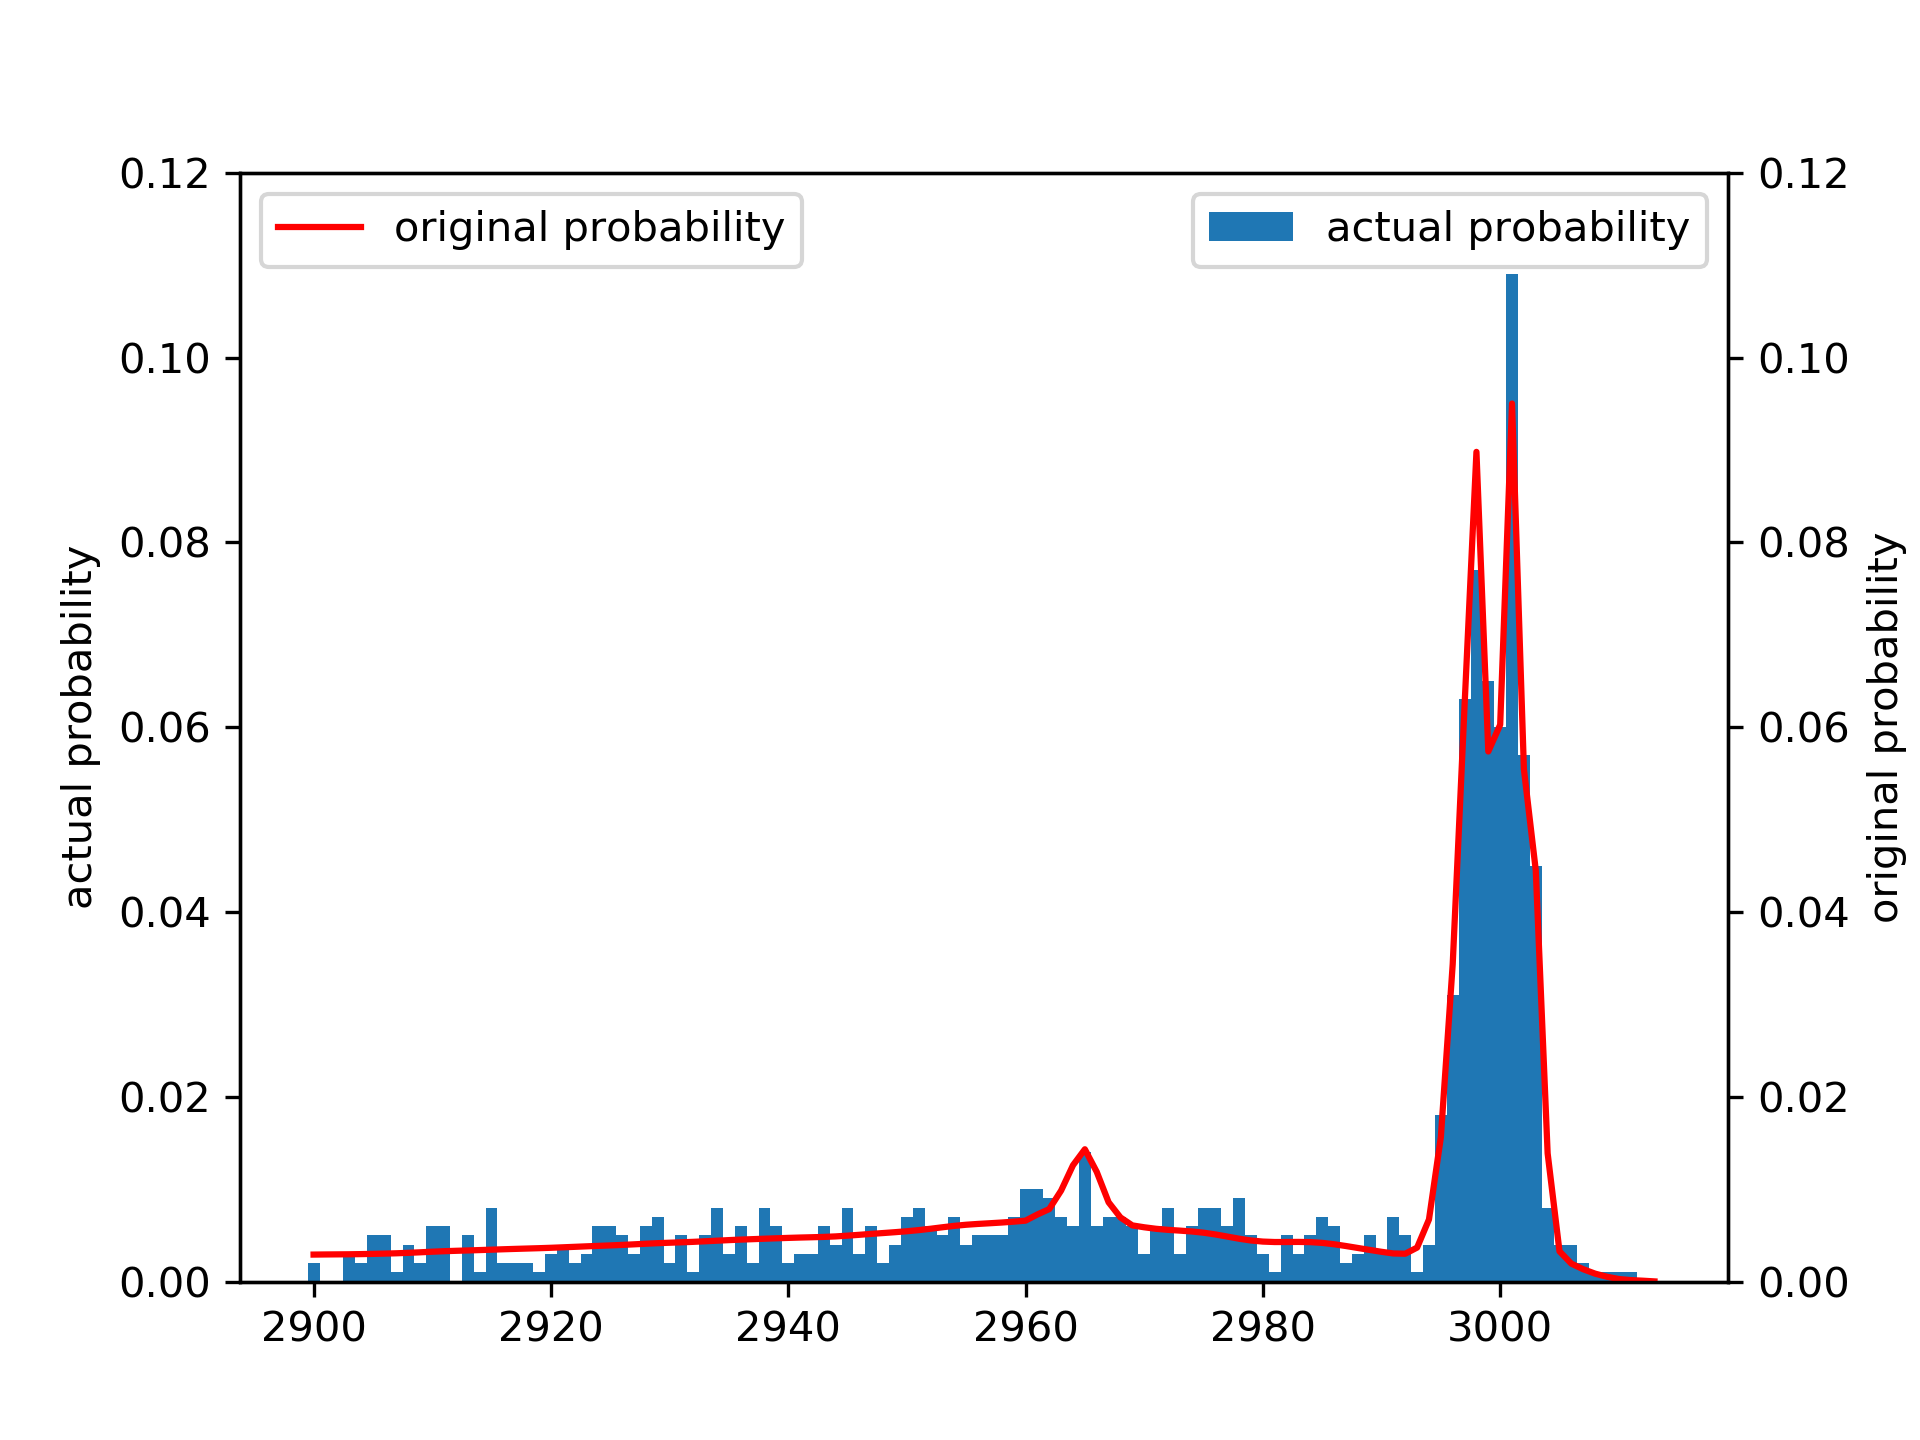
\includegraphics[width=10cm]  {c103.png}}        
\caption{\label{1} 舍选法$10^{3}$个点得到的概率分布与给定分布的比较}      
\end{figure}

\begin{figure}[!htbp]        
\center{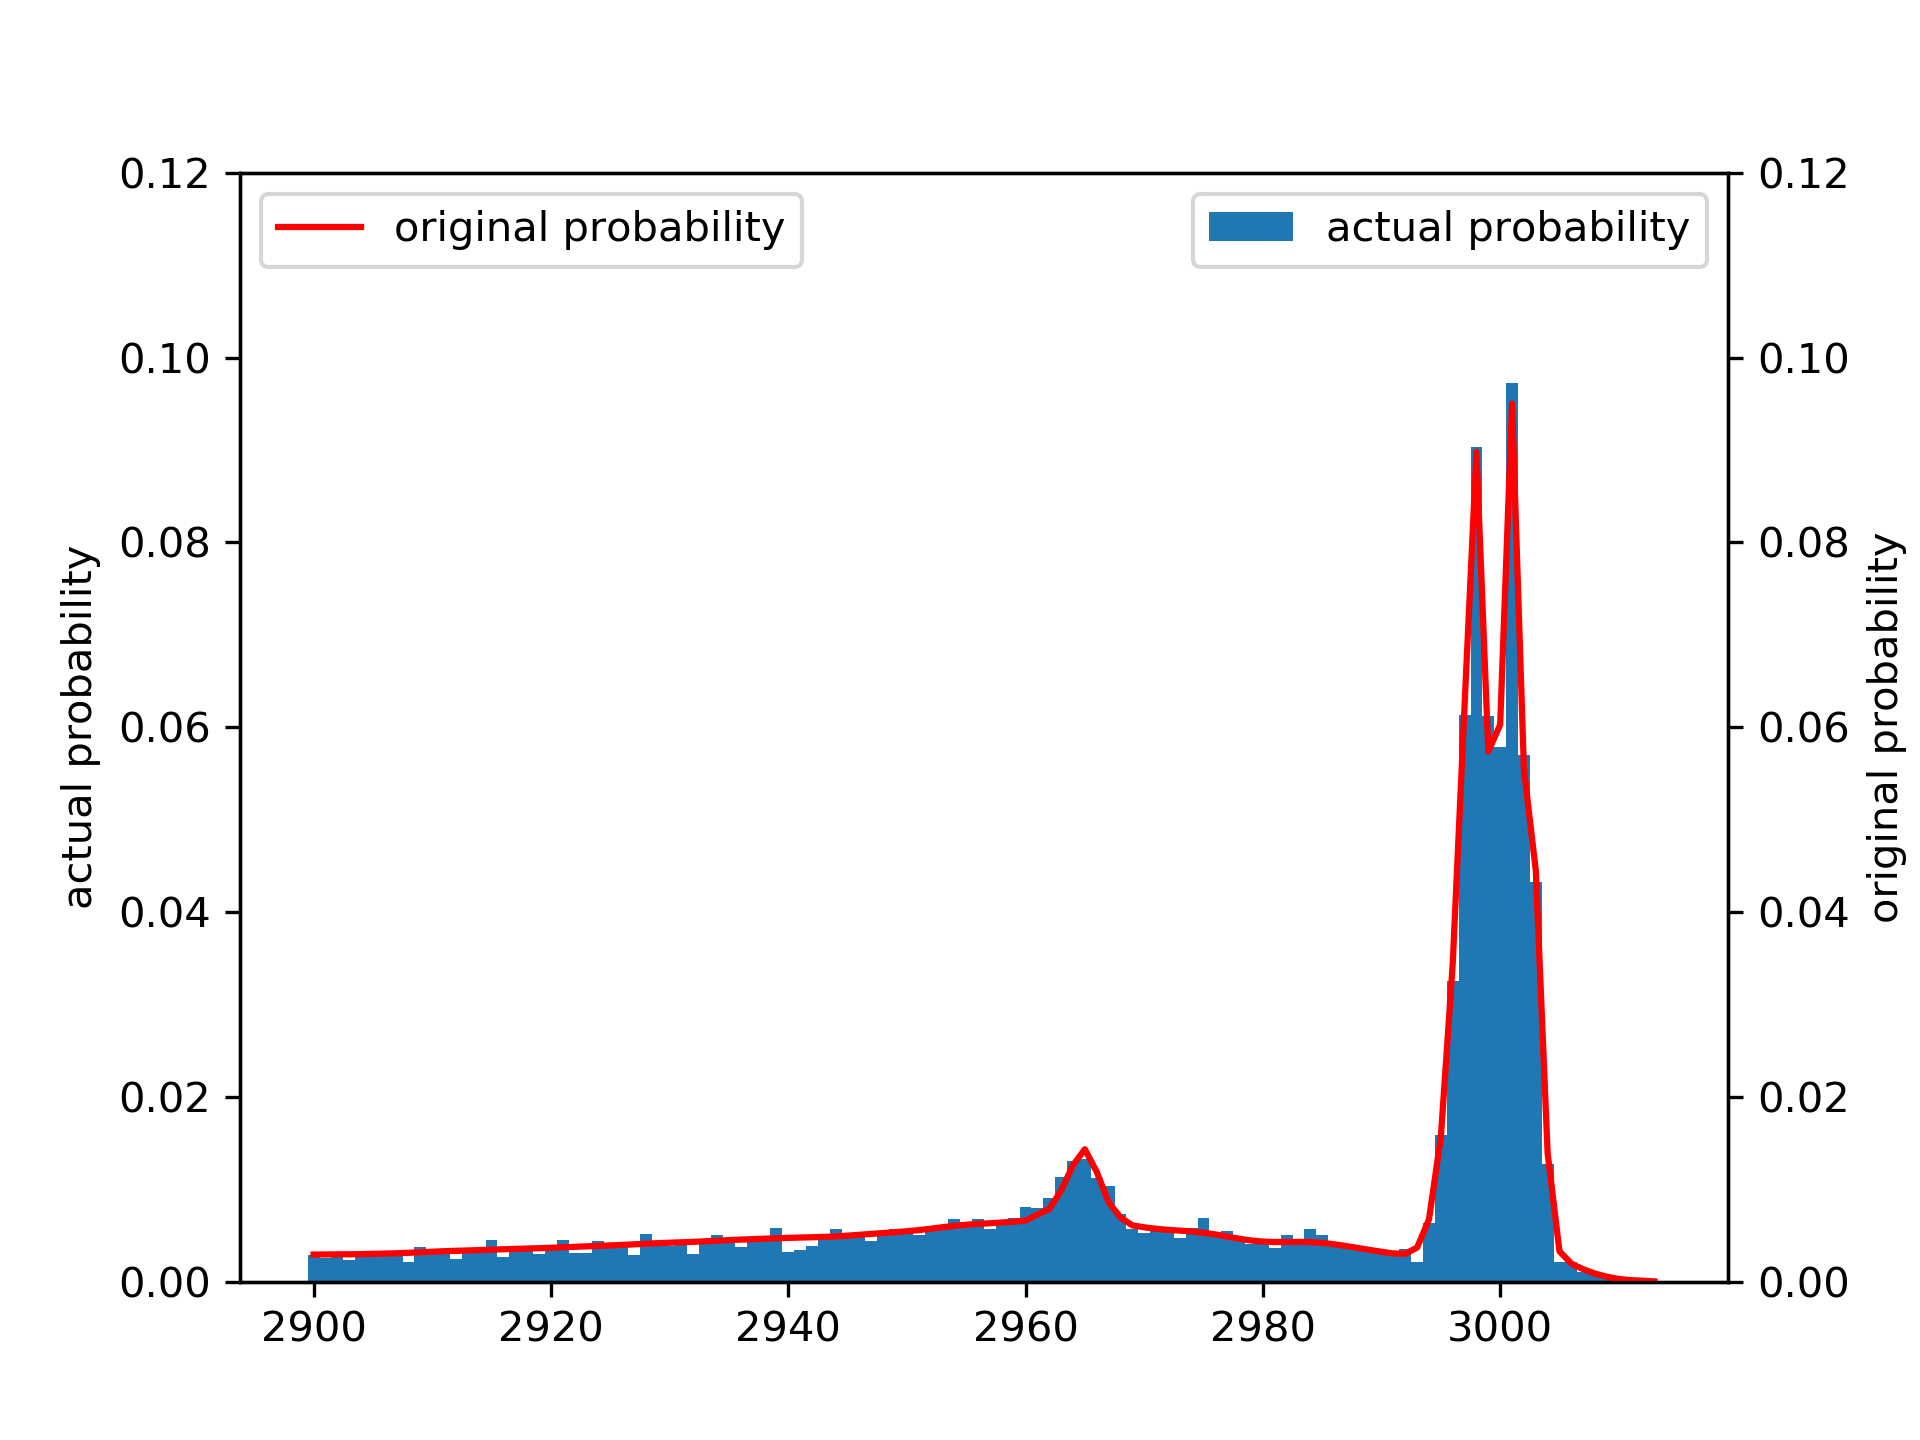
\includegraphics[width=10cm]  {c104.png}}        
\caption{\label{1} 舍选法$10^{4}$个点得到的概率分布与给定分布的比较}      
\end{figure}

\begin{figure}[!htbp]        
\center{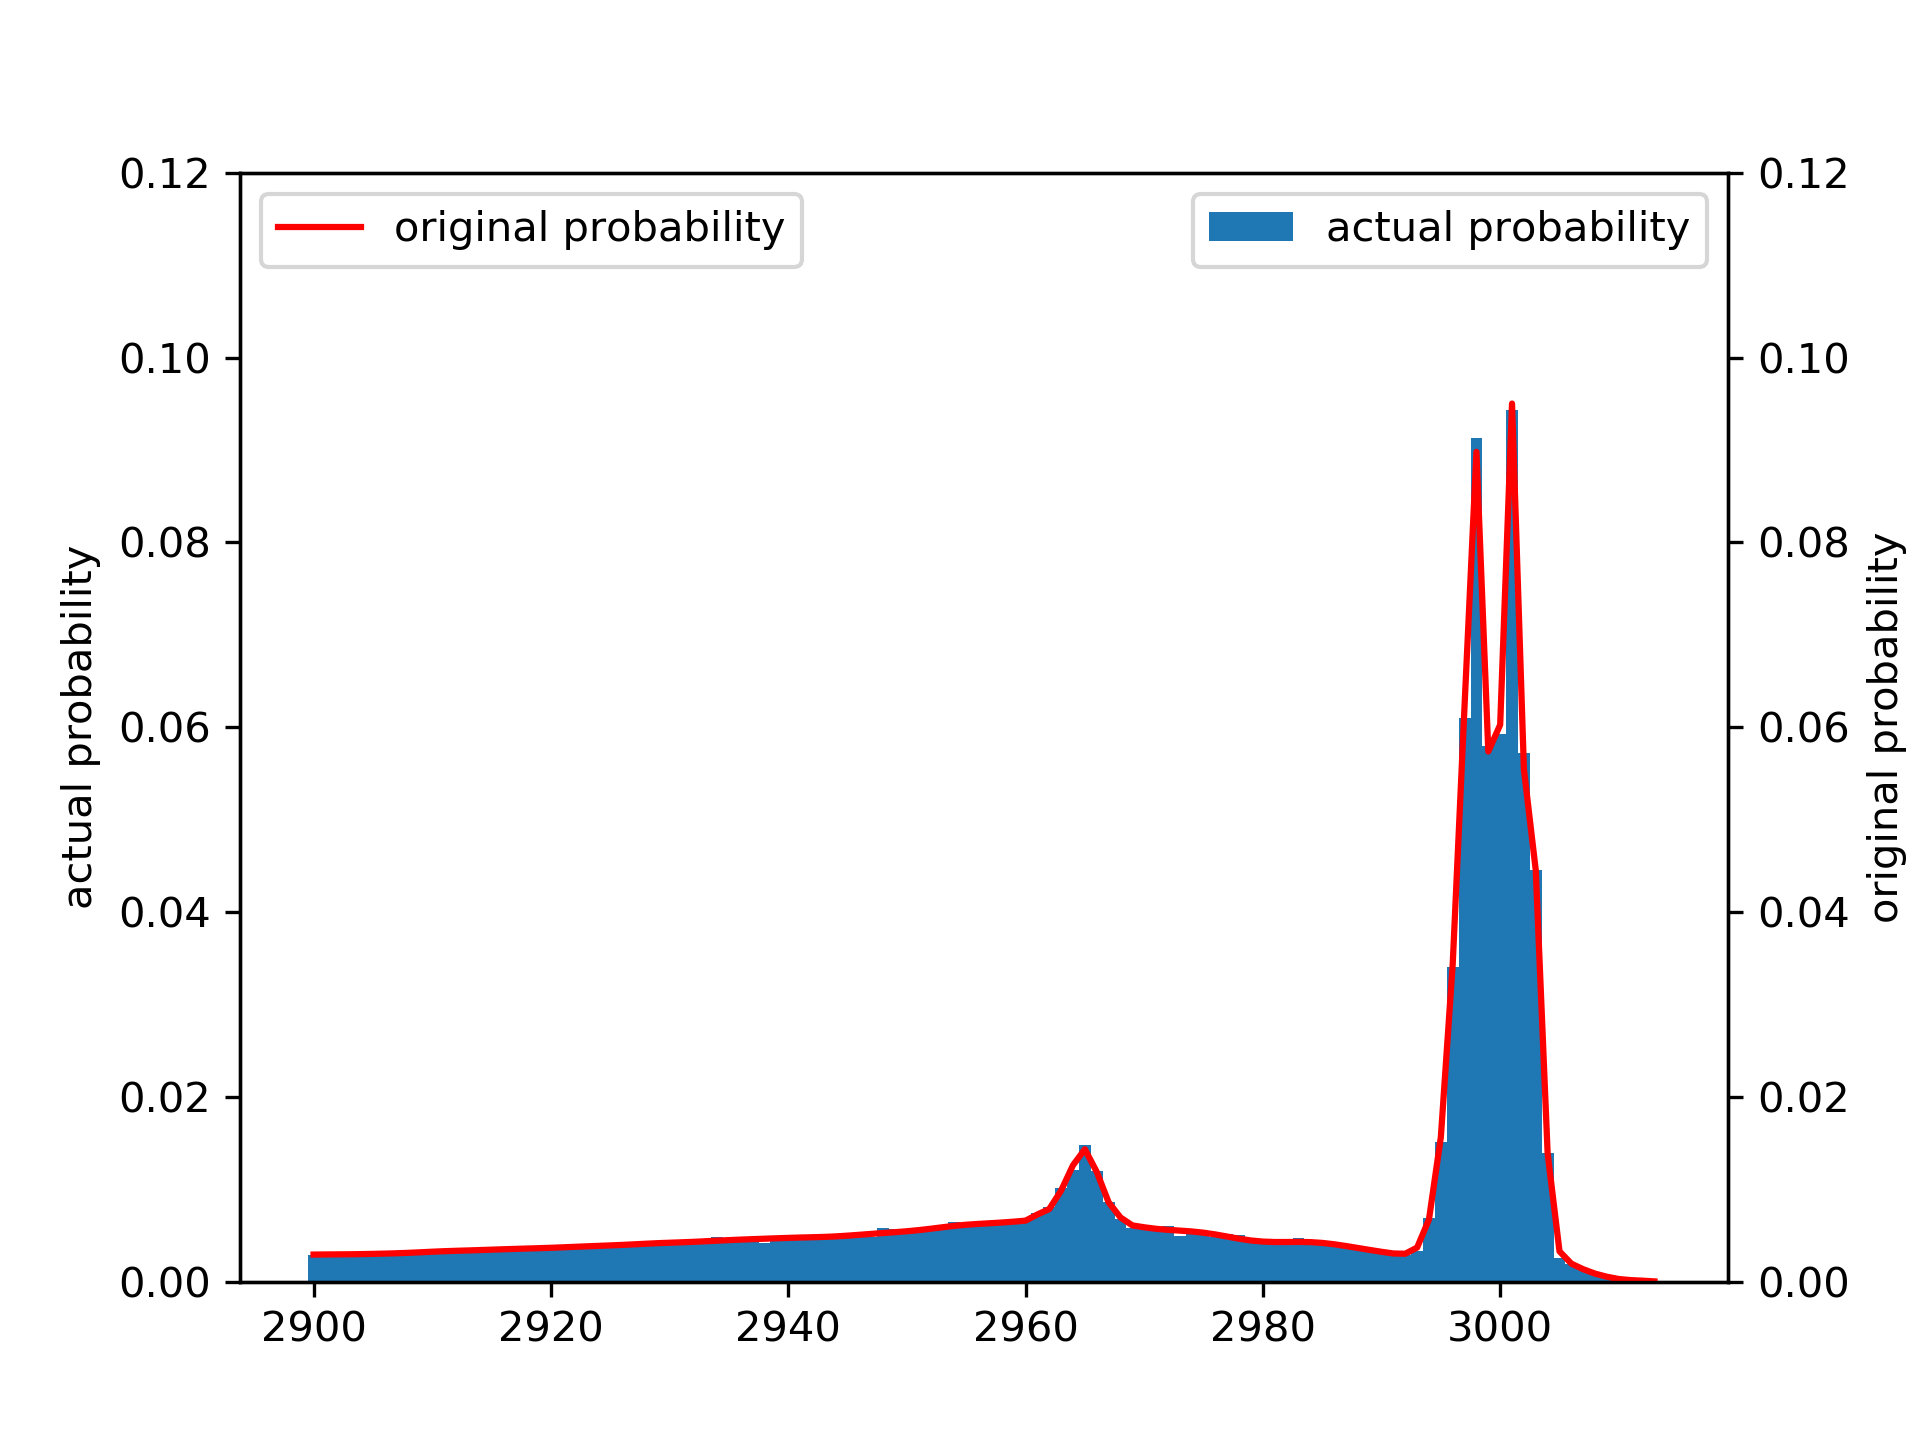
\includegraphics[width=10cm]  {c105.png}}        
\caption{\label{1} 舍选法$10^{5}$个点得到的概率分布与给定分布的比较}      
\end{figure}

\begin{figure}[!htbp]        
\center{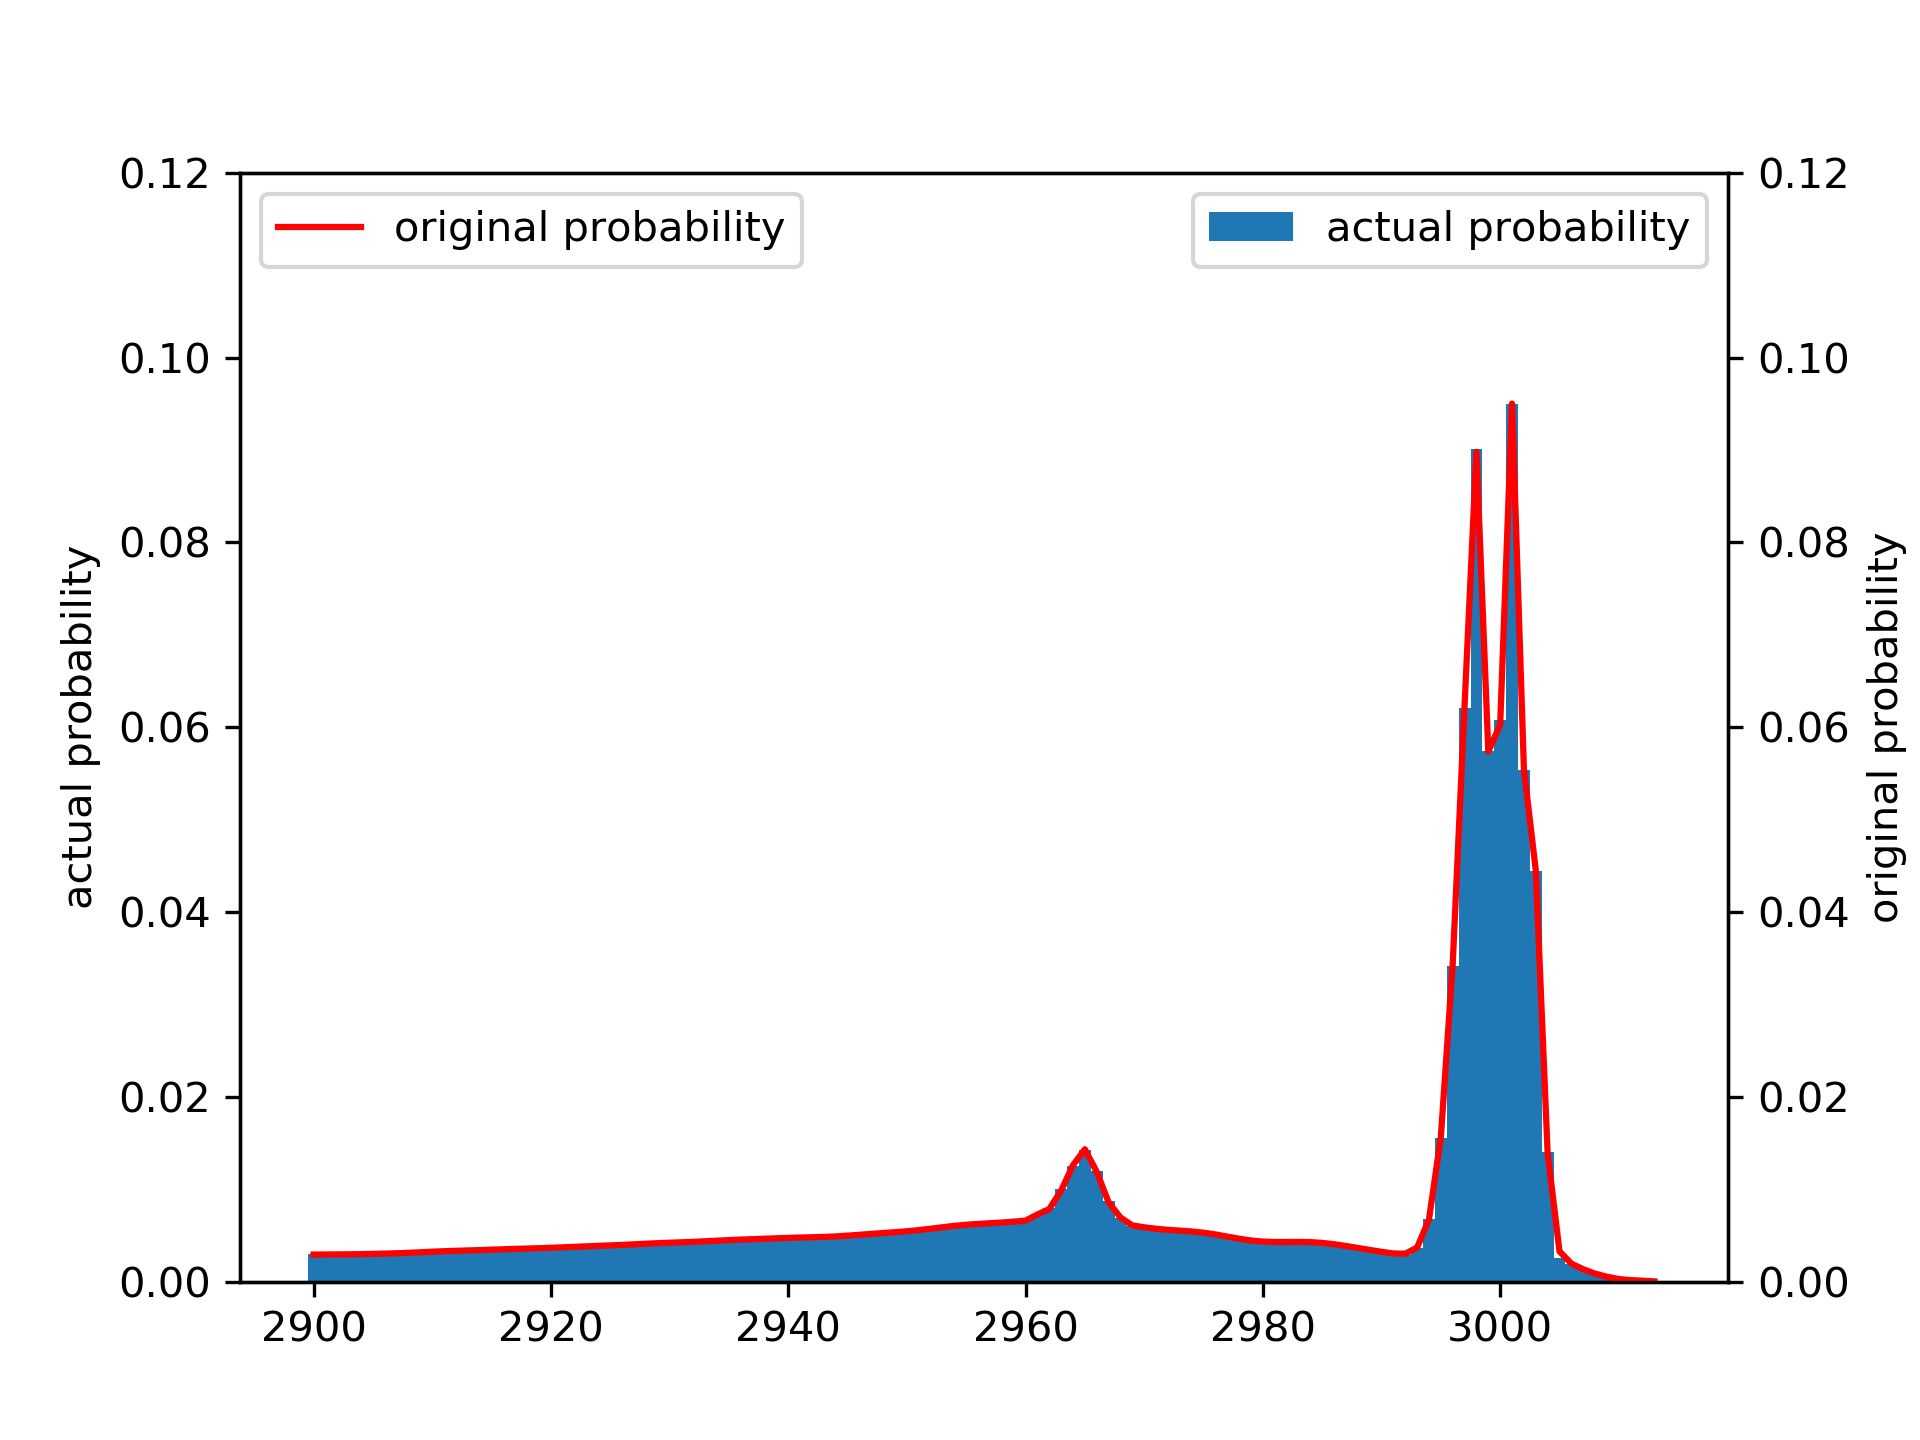
\includegraphics[width=10cm]  {c106.png}}        
\caption{\label{1} 舍选法$10^{6}$个点得到的概率分布与给定分布的比较}      
\end{figure}

\begin{figure}[!htbp]        
\center{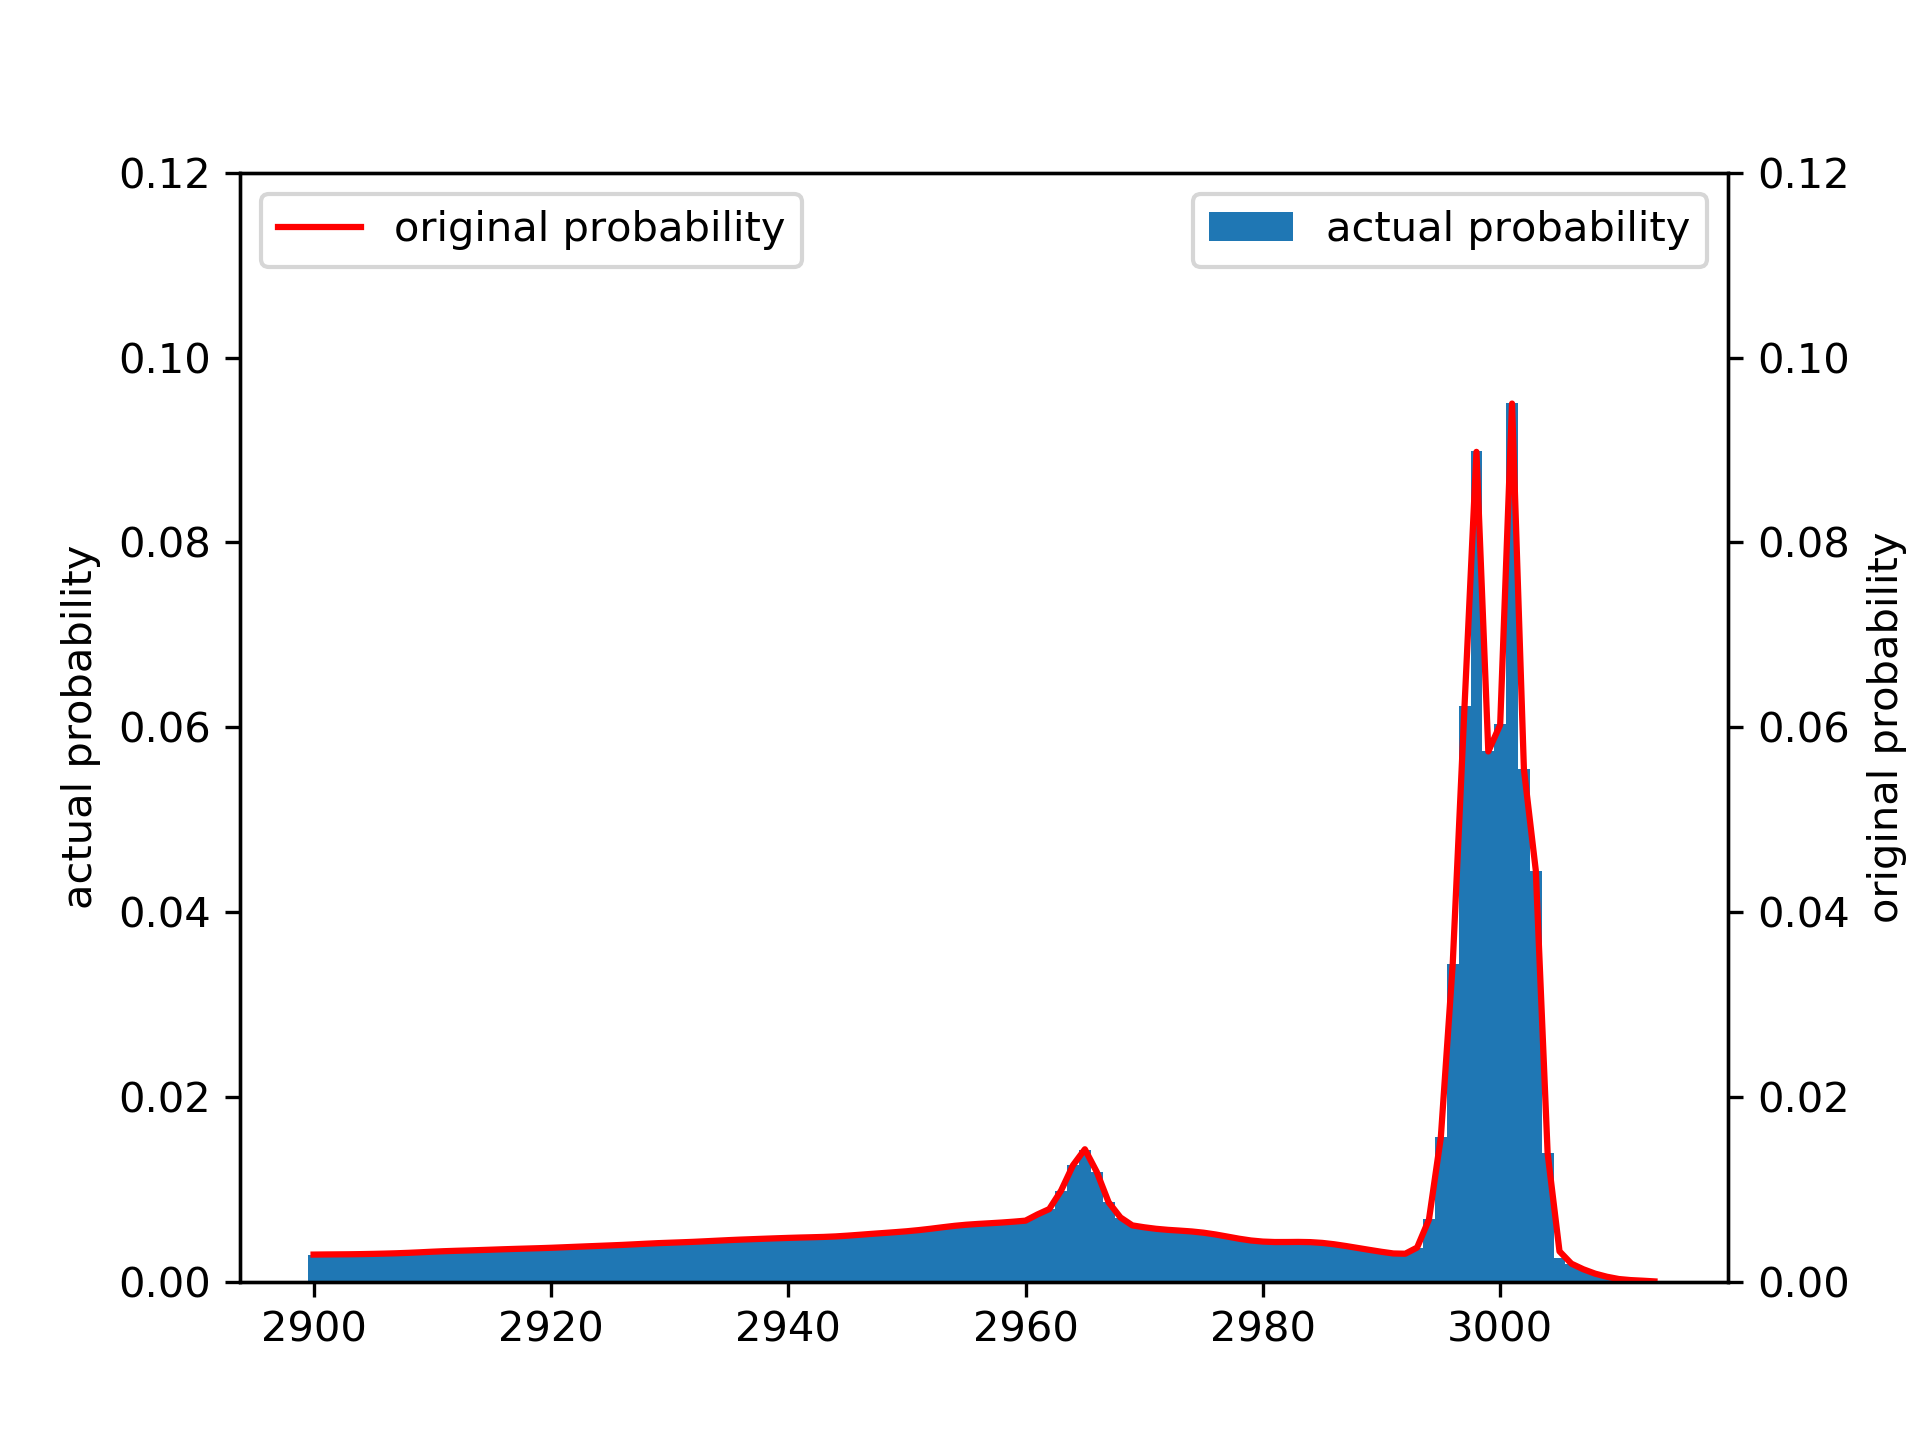
\includegraphics[width=10cm]  {c107.png}}        
\caption{\label{1} 舍选法$10^{7}$个点得到的概率分布与给定分布的比较}      
\end{figure}

\newpage 舍选法的抽样效率:

\begin{table}[!htbp]
\centering
\resizebox{\textwidth}{!}{
\begin{tabular}{|c|c|c|c|c|c|c|}
\hline

&$N=10^{2}$  &$N=10^{3}$  &$N=10^{4}$  &$N=10^{5}$  &$N=10^{6}$
&$N=10^{7}$  \\ \hline

抽样效率 &0.384615 &0.417711 &0.421799 &0.412528 &0.413363 &0.412934 \\ \hline

\end{tabular}}
\caption{抽样效率一览表}
\end{table}

从图中可以看出,不管是哪种抽样方法,在抽样点数变多时,抽样出来的点的概率分布都会收敛到给定概率分布。而直接抽样法的抽样效率永远为1;舍选抽样法的抽样效率永远都小于1,换取不同的比较函数可能会提高抽样效率,但相应的比较函数的抽样可能会变得很复杂,浪费编程的时间,在点数不是很多时,利用简单的分段函数作为比较函数会比较有效率。



\section{心得与体会}
通过此次作业结果,发现不管是直接抽样还是舍选法都能抽出以给定概率分布的点。也联系了对于离散点的抽样方法。
通过编程作业,也更加熟悉了一些C语言和\LaTeX 。

\newpage
\section{附录}

\begin{appendices}


\section{C语言程序源码}

\begin{lstlisting}[language = C]
#include <stdio.h>
#include <stdlib.h>
#include <math.h>
#define a 16807
#define m 2147483647
#define b 0
#define r (m%a)
#define q (m/a)
#define k 114 //能量取值个数

//写文件子程序,输入写成文件名称字符串str,数据来源于数组num,数据总数n
int my_filewriter_double(char str[],double num[],int n){
    FILE * fp;
    fp = fopen(str,"w+");

    for(int i=0;i<(n-1);i++)
    {
        fprintf(fp,"%lf,",num[i]);

    }
    fprintf(fp,"%lf",num[n-1]);    //最后一个数据后不加 ","
    fclose(fp);
    return 0;
}


//写文件子程序,输入写成文件名称字符串str,数据来源于数组num,数据总数n
int my_filewriter_int(char str[],int num[],int n){
    FILE * fp;
    fp = fopen(str,"w+");

    for(int i=0;i<(n-1);i++)
    {
        fprintf(fp,"%d,",num[i]);

    }
    fprintf(fp,"%d",num[n-1]);    //最后一个数据后不加 ","
    fclose(fp);
    return 0;
}





int my_filereader_int(char str[],int num[],int n){
    FILE * fp;
    int N = 0;
    
    if ((fp = fopen(str, "r")) == NULL) {
        printf("Have problem with opening the data file!\n");
        return 1;
    }
    
    int x;
    char buff[20];
    fgets(buff,20, fp); //先读取第一行表头

    for(int i=0;i<n;i++)
    {
        fscanf(fp,"%d",&x);
        fscanf(fp,"%d",&num[i]);
        N += num[i];
    }
    fclose(fp);
    return N;
}



// 16807 之 Schrage 方法产生随机数
int my_schrage(double ran[],int seed,int n){
    for (int i = 0; i < n - 1; i++) {
        if (seed >= 0) {
            ran[i] = seed / (double) m;
        } else {
            ran[i] = (seed + m) / (double) m;
        }
        if(seed == m-1){
            if(a >=  b){    //由于Schrage方法只对z in (0,m-1)成立,故这里要讨论z == m-1的情况
                seed = m + (b-a) % m;
            }
            else   seed =  (b-a) % m;

        }
        else seed = ((a * (seed % q) - r * (seed /  q)) + b % m ) % m;  //递推式
    }
    if (seed >= 0) {
        ran[n-1] = seed / (double) m;
    } else {
        ran[n-1] = (seed + m) / (double) m;
    }
    return 0;
}




// 舍选法抽样
int  my_choose(int seed[], int ran[],double orip[], int n){
    double x;
    double y;
    int flag = 0;  //记录总抽样次数
    for (int j = 0; j <= n; ) {  //j记录舍选成功的次数
        flag++;
        
        if (seed[0] >= 0) {   //产生在[0,2,4199]间均匀抽取的\xi
            x =  2.41994*(seed[0] / (double)m) ;
        }
        else{
            x = 2.41994*((seed[0] + m) / (double)m) ;
        }
        
        if (seed[1] >= 0) {   //产生在[0,1]间均匀抽取的\eta
            y =  (seed[1] / (double)m);
        }
        else{
            y =  ((seed[1] + m) / (double)m);
        }
        if(x <= 1.3536) {   //对于不同区级的\xi对x,y分别赋值
            x = x/0.0144 + 2900;
            y = y*0.0144;
        }
        else if(x <= 2.3997 && x > 1.3536) {
            x = (x-1.3536)/0.0951 + 2994;
            y = y*0.0951;
        }
        else {
            x = (x-2.3997)/0.00253 + 3005;
            y = y*0.00253;
        }
        
        if( y <= orip[(int)floor(x-2900)] ){ //舍选条件判断
           j++;
           ran[j] = (int)floor(x);
        }//满足舍选法条件后写入数据
        seed[0] = ((a * (seed[0] % q) - r * (seed[0] /  q)) + b % m ) % m;
        seed[1] = ((a * (seed[1] % q) - r * (seed[1] /  q)) + b % m ) % m;
        if(seed[0] == m-1){
            if(a >=  b){    //由于Schrage方法只对z in (0,m-1)成立,故这里要讨论z == m-1的情况
                seed[0] = m + (b-a) % m;
            }
            else   seed[0] =  (b-a) % m;
            
        }
        if(seed[1] == m-1){
            if(a >=  b){    //由于Schrage方法只对z in (0,m-1)成立,故这里要讨论z == m-1的情况
                seed[1] = m + (b-a) % m;
            }
            else   seed[1] =  (b-a) % m;
            
        }
    }
    return flag;
}






int main(int argc, const char * argv[]) {
    int x[k];
    double p[k];  //存放给定数据的的不同x对应的抽到的概率
    double E[k];  //存放抽样得到的数据的不同x对应的抽到的概率
    int flag;  //舍选法总抽样次数
    int seed[2] = {34028207,1677078722};   //舍选法利用的16807方法所需的初始2种子
    for(int i=0;i<k;i++){  //初始化
        E[i] = 0;
    }
    int N;   //给定数据的计数总数
    N = my_filereader_int("data.txt", x, k);
    for(int i=0;i<k;i++){
        p[i] = (double)x[i]/N;
    }
    my_filewriter_double("orip.txt", p, k);  //输出给定数据的的不同x对应的抽到的概率
    
    
    char str[50];
    printf("请输入您所需要的总点数:");
    while (!scanf("%d",&N)) {   //简单的输入检查,此时N变为需要产生的随机点的总数
        gets(str);
        printf("\nInput error,please try again\n");
        printf("请输入您所需要的总点数:");
    }
    if(N >1000000) printf("您输入的参数已接受,正在计算请稍等片刻~\n");

    int *ran1 = malloc(sizeof(int) * N);  //用来存放舍选法产生的随机数
   
    flag = my_choose(seed, ran1, p, N);
    //my_filewriter_double("ran1,dat",ran1,N);  //可以输出舍选法抽样得到的数据,此处只计算得到数据的概率分布,故输出略去。
    
    for(int i = 0;i < N;i++){
        E[(int)floor(ran1[i]-2900)] += (double)1/N; //得到离散的x的取值
    }
    
    my_filewriter_double("p-1.txt", E, k);  //输出舍选法得到的数据的概率分布至文件
    printf("舍选法的抽样效率约为%lf\n",(double)N/flag);
    
    
    double * ran2 = malloc(sizeof(double) * N);  //直接抽样法所用的数据存放数组
    
    my_schrage(ran2, 1, N); //种子值设为1   //得到[0,1]均匀抽样的数据点
    
    for(int i=0;i<k;i++){  //初始化
        E[i] = 0;
    }
    
    for(int i=0;i<N;i++){   //离散数据的直接抽样法
        double sump = 0;
        for (int j=0;j<k;j++){
            sump += p[j];
            if(ran2[i] < sump) {
                ran2[i] = j + 2900;
                E[j] += (double)1/N;
                break;
            }
        }
    }
    
    //my_filewriter_double("ran2.dat",ran2,N);  //可以输出直接抽样法抽样得到的数据,此处只计算得到数据的概率分布,故输出略去。
    my_filewriter_double("p-2.txt", E, k);
    
    return 0;
}
\end{lstlisting}

\section{可视化python源程序}[language=python]

\begin{lstlisting}
	
import matplotlib.pyplot as plt
from mpl_toolkits.mplot3d import Axes3D
import numpy as np
#from IPython.core.pylabtools import figsize # import figsize
#figsize(12.5, 4) # 设置 figsize
plt.rcParams['savefig.dpi'] = 300 #图片像素
plt.rcParams['figure.dpi'] = 300 #分辨率
# 默认的像素:[6.0,4.0],分辨率为100,图片尺寸为 600&400
fig = plt.figure()
ax1 = fig.add_subplot(111)

with open('problem 7/F.txt', 'r') as f:
    while True:
        lines = f.readline() # 整行读取数据
        if not lines:
            break
        Y = [float(i) for i in lines.split(',')] # 将整行数据分割处理
    Y = np.array(Y) # 将数据从list类型转换为array类型。


with open('problem 7/orip.txt', 'r') as f:
    while True:
        lines = f.readline() # 整行读取数据
        if not lines:
            break
        oY = [float(i) for i in lines.split(',')] # 将整行数据分割处理
    oY = np.array(oY)  # 将数据从list类型转换为array类型。


X = np.arange(2900, 3014)


plt.bar(x=X, height=Y, width=1, label='actual probability')
ax1.legend(loc=1)
ax1.set_ylabel('actual probability')
ax1.set_ylim([0, 0.12])

ax2 = ax1.twinx()

ax2.plot(X, oY, 'r', label='original probability')
ax2.legend(loc=2)
ax2.set_ylabel('original probability')
ax2.set_ylim([0, 0.12])

plt.xlabel('Energy')


plt.savefig("1.png")

	
\end{lstlisting}

\end{appendices}




\end{document}
